% Options for packages loaded elsewhere
\PassOptionsToPackage{unicode}{hyperref}
\PassOptionsToPackage{hyphens}{url}
%
\documentclass[
]{article}
\usepackage{amsmath,amssymb}
\usepackage{lmodern}
\usepackage{iftex}
\ifPDFTeX
  \usepackage[T1]{fontenc}
  \usepackage[utf8]{inputenc}
  \usepackage{textcomp} % provide euro and other symbols
\else % if luatex or xetex
  \usepackage{unicode-math}
  \defaultfontfeatures{Scale=MatchLowercase}
  \defaultfontfeatures[\rmfamily]{Ligatures=TeX,Scale=1}
\fi
% Use upquote if available, for straight quotes in verbatim environments
\IfFileExists{upquote.sty}{\usepackage{upquote}}{}
\IfFileExists{microtype.sty}{% use microtype if available
  \usepackage[]{microtype}
  \UseMicrotypeSet[protrusion]{basicmath} % disable protrusion for tt fonts
}{}
\makeatletter
\@ifundefined{KOMAClassName}{% if non-KOMA class
  \IfFileExists{parskip.sty}{%
    \usepackage{parskip}
  }{% else
    \setlength{\parindent}{0pt}
    \setlength{\parskip}{6pt plus 2pt minus 1pt}}
}{% if KOMA class
  \KOMAoptions{parskip=half}}
\makeatother
\usepackage{xcolor}
\usepackage[margin=1in]{geometry}
\usepackage{color}
\usepackage{fancyvrb}
\newcommand{\VerbBar}{|}
\newcommand{\VERB}{\Verb[commandchars=\\\{\}]}
\DefineVerbatimEnvironment{Highlighting}{Verbatim}{commandchars=\\\{\}}
% Add ',fontsize=\small' for more characters per line
\usepackage{framed}
\definecolor{shadecolor}{RGB}{248,248,248}
\newenvironment{Shaded}{\begin{snugshade}}{\end{snugshade}}
\newcommand{\AlertTok}[1]{\textcolor[rgb]{0.94,0.16,0.16}{#1}}
\newcommand{\AnnotationTok}[1]{\textcolor[rgb]{0.56,0.35,0.01}{\textbf{\textit{#1}}}}
\newcommand{\AttributeTok}[1]{\textcolor[rgb]{0.77,0.63,0.00}{#1}}
\newcommand{\BaseNTok}[1]{\textcolor[rgb]{0.00,0.00,0.81}{#1}}
\newcommand{\BuiltInTok}[1]{#1}
\newcommand{\CharTok}[1]{\textcolor[rgb]{0.31,0.60,0.02}{#1}}
\newcommand{\CommentTok}[1]{\textcolor[rgb]{0.56,0.35,0.01}{\textit{#1}}}
\newcommand{\CommentVarTok}[1]{\textcolor[rgb]{0.56,0.35,0.01}{\textbf{\textit{#1}}}}
\newcommand{\ConstantTok}[1]{\textcolor[rgb]{0.00,0.00,0.00}{#1}}
\newcommand{\ControlFlowTok}[1]{\textcolor[rgb]{0.13,0.29,0.53}{\textbf{#1}}}
\newcommand{\DataTypeTok}[1]{\textcolor[rgb]{0.13,0.29,0.53}{#1}}
\newcommand{\DecValTok}[1]{\textcolor[rgb]{0.00,0.00,0.81}{#1}}
\newcommand{\DocumentationTok}[1]{\textcolor[rgb]{0.56,0.35,0.01}{\textbf{\textit{#1}}}}
\newcommand{\ErrorTok}[1]{\textcolor[rgb]{0.64,0.00,0.00}{\textbf{#1}}}
\newcommand{\ExtensionTok}[1]{#1}
\newcommand{\FloatTok}[1]{\textcolor[rgb]{0.00,0.00,0.81}{#1}}
\newcommand{\FunctionTok}[1]{\textcolor[rgb]{0.00,0.00,0.00}{#1}}
\newcommand{\ImportTok}[1]{#1}
\newcommand{\InformationTok}[1]{\textcolor[rgb]{0.56,0.35,0.01}{\textbf{\textit{#1}}}}
\newcommand{\KeywordTok}[1]{\textcolor[rgb]{0.13,0.29,0.53}{\textbf{#1}}}
\newcommand{\NormalTok}[1]{#1}
\newcommand{\OperatorTok}[1]{\textcolor[rgb]{0.81,0.36,0.00}{\textbf{#1}}}
\newcommand{\OtherTok}[1]{\textcolor[rgb]{0.56,0.35,0.01}{#1}}
\newcommand{\PreprocessorTok}[1]{\textcolor[rgb]{0.56,0.35,0.01}{\textit{#1}}}
\newcommand{\RegionMarkerTok}[1]{#1}
\newcommand{\SpecialCharTok}[1]{\textcolor[rgb]{0.00,0.00,0.00}{#1}}
\newcommand{\SpecialStringTok}[1]{\textcolor[rgb]{0.31,0.60,0.02}{#1}}
\newcommand{\StringTok}[1]{\textcolor[rgb]{0.31,0.60,0.02}{#1}}
\newcommand{\VariableTok}[1]{\textcolor[rgb]{0.00,0.00,0.00}{#1}}
\newcommand{\VerbatimStringTok}[1]{\textcolor[rgb]{0.31,0.60,0.02}{#1}}
\newcommand{\WarningTok}[1]{\textcolor[rgb]{0.56,0.35,0.01}{\textbf{\textit{#1}}}}
\usepackage{graphicx}
\makeatletter
\def\maxwidth{\ifdim\Gin@nat@width>\linewidth\linewidth\else\Gin@nat@width\fi}
\def\maxheight{\ifdim\Gin@nat@height>\textheight\textheight\else\Gin@nat@height\fi}
\makeatother
% Scale images if necessary, so that they will not overflow the page
% margins by default, and it is still possible to overwrite the defaults
% using explicit options in \includegraphics[width, height, ...]{}
\setkeys{Gin}{width=\maxwidth,height=\maxheight,keepaspectratio}
% Set default figure placement to htbp
\makeatletter
\def\fps@figure{htbp}
\makeatother
\setlength{\emergencystretch}{3em} % prevent overfull lines
\providecommand{\tightlist}{%
  \setlength{\itemsep}{0pt}\setlength{\parskip}{0pt}}
\setcounter{secnumdepth}{-\maxdimen} % remove section numbering
\ifLuaTeX
  \usepackage{selnolig}  % disable illegal ligatures
\fi
\IfFileExists{bookmark.sty}{\usepackage{bookmark}}{\usepackage{hyperref}}
\IfFileExists{xurl.sty}{\usepackage{xurl}}{} % add URL line breaks if available
\urlstyle{same} % disable monospaced font for URLs
\hypersetup{
  hidelinks,
  pdfcreator={LaTeX via pandoc}}

\author{}
\date{\vspace{-2.5em}}

\begin{document}

\begin{Shaded}
\begin{Highlighting}[]
\FunctionTok{library}\NormalTok{(binom)}
\FunctionTok{library}\NormalTok{(car)}
\end{Highlighting}
\end{Shaded}

\begin{verbatim}
## Loading required package: carData
\end{verbatim}

\begin{Shaded}
\begin{Highlighting}[]
\FunctionTok{library}\NormalTok{(collapsibleTree)}
\FunctionTok{library}\NormalTok{(dbplyr)}
\FunctionTok{library}\NormalTok{(dplyr)}
\end{Highlighting}
\end{Shaded}

\begin{verbatim}
## 
## Attaching package: 'dplyr'
\end{verbatim}

\begin{verbatim}
## The following objects are masked from 'package:dbplyr':
## 
##     ident, sql
\end{verbatim}

\begin{verbatim}
## The following object is masked from 'package:car':
## 
##     recode
\end{verbatim}

\begin{verbatim}
## The following objects are masked from 'package:stats':
## 
##     filter, lag
\end{verbatim}

\begin{verbatim}
## The following objects are masked from 'package:base':
## 
##     intersect, setdiff, setequal, union
\end{verbatim}

\begin{Shaded}
\begin{Highlighting}[]
\FunctionTok{library}\NormalTok{(EnvStats)}
\end{Highlighting}
\end{Shaded}

\begin{verbatim}
## 
## Attaching package: 'EnvStats'
\end{verbatim}

\begin{verbatim}
## The following object is masked from 'package:car':
## 
##     qqPlot
\end{verbatim}

\begin{verbatim}
## The following objects are masked from 'package:stats':
## 
##     predict, predict.lm
\end{verbatim}

\begin{verbatim}
## The following object is masked from 'package:base':
## 
##     print.default
\end{verbatim}

\begin{Shaded}
\begin{Highlighting}[]
\FunctionTok{library}\NormalTok{(ggformula)}
\end{Highlighting}
\end{Shaded}

\begin{verbatim}
## Loading required package: ggplot2
\end{verbatim}

\begin{verbatim}
## Loading required package: ggstance
\end{verbatim}

\begin{verbatim}
## 
## Attaching package: 'ggstance'
\end{verbatim}

\begin{verbatim}
## The following objects are masked from 'package:ggplot2':
## 
##     geom_errorbarh, GeomErrorbarh
\end{verbatim}

\begin{verbatim}
## Loading required package: scales
\end{verbatim}

\begin{verbatim}
## Loading required package: ggridges
\end{verbatim}

\begin{verbatim}
## 
## New to ggformula?  Try the tutorials: 
##  learnr::run_tutorial("introduction", package = "ggformula")
##  learnr::run_tutorial("refining", package = "ggformula")
\end{verbatim}

\begin{Shaded}
\begin{Highlighting}[]
\FunctionTok{library}\NormalTok{(ggplot2)}
\FunctionTok{library}\NormalTok{(gmodels)}
\FunctionTok{library}\NormalTok{(htmltools)}
\FunctionTok{library}\NormalTok{(ISLR)}
\FunctionTok{library}\NormalTok{(knitr)}
\FunctionTok{library}\NormalTok{(lawstat)}
\end{Highlighting}
\end{Shaded}

\begin{verbatim}
## 
## Attaching package: 'lawstat'
\end{verbatim}

\begin{verbatim}
## The following object is masked from 'package:car':
## 
##     levene.test
\end{verbatim}

\begin{Shaded}
\begin{Highlighting}[]
\FunctionTok{library}\NormalTok{(markdown)}
\FunctionTok{library}\NormalTok{(mosaic)}
\end{Highlighting}
\end{Shaded}

\begin{verbatim}
## Registered S3 method overwritten by 'mosaic':
##   method                           from   
##   fortify.SpatialPolygonsDataFrame ggplot2
\end{verbatim}

\begin{verbatim}
## 
## The 'mosaic' package masks several functions from core packages in order to add 
## additional features.  The original behavior of these functions should not be affected by this.
\end{verbatim}

\begin{verbatim}
## 
## Attaching package: 'mosaic'
\end{verbatim}

\begin{verbatim}
## The following object is masked from 'package:Matrix':
## 
##     mean
\end{verbatim}

\begin{verbatim}
## The following object is masked from 'package:scales':
## 
##     rescale
\end{verbatim}

\begin{verbatim}
## The following object is masked from 'package:ggplot2':
## 
##     stat
\end{verbatim}

\begin{verbatim}
## The following object is masked from 'package:EnvStats':
## 
##     iqr
\end{verbatim}

\begin{verbatim}
## The following objects are masked from 'package:dplyr':
## 
##     count, do, tally
\end{verbatim}

\begin{verbatim}
## The following objects are masked from 'package:car':
## 
##     deltaMethod, logit
\end{verbatim}

\begin{verbatim}
## The following objects are masked from 'package:stats':
## 
##     binom.test, cor, cor.test, cov, fivenum, IQR, median, prop.test,
##     quantile, sd, t.test, var
\end{verbatim}

\begin{verbatim}
## The following objects are masked from 'package:base':
## 
##     max, mean, min, prod, range, sample, sum
\end{verbatim}

\begin{Shaded}
\begin{Highlighting}[]
\FunctionTok{library}\NormalTok{(mdsr)}
\FunctionTok{library}\NormalTok{(mosaicData)}
\FunctionTok{library}\NormalTok{(nycflights13)}
\FunctionTok{library}\NormalTok{(olsrr)}
\end{Highlighting}
\end{Shaded}

\begin{verbatim}
## 
## Attaching package: 'olsrr'
\end{verbatim}

\begin{verbatim}
## The following object is masked from 'package:datasets':
## 
##     rivers
\end{verbatim}

\begin{Shaded}
\begin{Highlighting}[]
\FunctionTok{library}\NormalTok{(plyr)}
\end{Highlighting}
\end{Shaded}

\begin{verbatim}
## ------------------------------------------------------------------------------
\end{verbatim}

\begin{verbatim}
## You have loaded plyr after dplyr - this is likely to cause problems.
## If you need functions from both plyr and dplyr, please load plyr first, then dplyr:
## library(plyr); library(dplyr)
\end{verbatim}

\begin{verbatim}
## ------------------------------------------------------------------------------
\end{verbatim}

\begin{verbatim}
## 
## Attaching package: 'plyr'
\end{verbatim}

\begin{verbatim}
## The following object is masked from 'package:mosaic':
## 
##     count
\end{verbatim}

\begin{verbatim}
## The following objects are masked from 'package:dplyr':
## 
##     arrange, count, desc, failwith, id, mutate, rename, summarise,
##     summarize
\end{verbatim}

\begin{Shaded}
\begin{Highlighting}[]
\FunctionTok{library}\NormalTok{(purrr)}
\end{Highlighting}
\end{Shaded}

\begin{verbatim}
## 
## Attaching package: 'purrr'
\end{verbatim}

\begin{verbatim}
## The following object is masked from 'package:plyr':
## 
##     compact
\end{verbatim}

\begin{verbatim}
## The following object is masked from 'package:mosaic':
## 
##     cross
\end{verbatim}

\begin{verbatim}
## The following object is masked from 'package:scales':
## 
##     discard
\end{verbatim}

\begin{verbatim}
## The following object is masked from 'package:car':
## 
##     some
\end{verbatim}

\begin{Shaded}
\begin{Highlighting}[]
\FunctionTok{library}\NormalTok{(plotly)}
\end{Highlighting}
\end{Shaded}

\begin{verbatim}
## 
## Attaching package: 'plotly'
\end{verbatim}

\begin{verbatim}
## The following objects are masked from 'package:plyr':
## 
##     arrange, mutate, rename, summarise
\end{verbatim}

\begin{verbatim}
## The following object is masked from 'package:mosaic':
## 
##     do
\end{verbatim}

\begin{verbatim}
## The following object is masked from 'package:ggplot2':
## 
##     last_plot
\end{verbatim}

\begin{verbatim}
## The following object is masked from 'package:stats':
## 
##     filter
\end{verbatim}

\begin{verbatim}
## The following object is masked from 'package:graphics':
## 
##     layout
\end{verbatim}

\begin{Shaded}
\begin{Highlighting}[]
\FunctionTok{library}\NormalTok{(resampledata)}
\end{Highlighting}
\end{Shaded}

\begin{verbatim}
## 
## Attaching package: 'resampledata'
\end{verbatim}

\begin{verbatim}
## The following object is masked from 'package:carData':
## 
##     Salaries
\end{verbatim}

\begin{verbatim}
## The following object is masked from 'package:datasets':
## 
##     Titanic
\end{verbatim}

\begin{Shaded}
\begin{Highlighting}[]
\FunctionTok{library}\NormalTok{(rmarkdown)}
\FunctionTok{library}\NormalTok{(rpart)}
\FunctionTok{library}\NormalTok{(rpart.plot)}
\FunctionTok{library}\NormalTok{(rvest)}
\FunctionTok{library}\NormalTok{(SDaA)}
\end{Highlighting}
\end{Shaded}

\begin{verbatim}
## 
## Attaching package: 'SDaA'
\end{verbatim}

\begin{verbatim}
## The following object is masked from 'package:plyr':
## 
##     ozone
\end{verbatim}

\begin{verbatim}
## The following object is masked from 'package:ggplot2':
## 
##     seals
\end{verbatim}

\begin{Shaded}
\begin{Highlighting}[]
\FunctionTok{library}\NormalTok{(shiny)}
\FunctionTok{library}\NormalTok{(stringi)}
\FunctionTok{library}\NormalTok{(tibble)}
\FunctionTok{library}\NormalTok{(tidyr)}
\end{Highlighting}
\end{Shaded}

\begin{verbatim}
## 
## Attaching package: 'tidyr'
\end{verbatim}

\begin{verbatim}
## The following objects are masked from 'package:Matrix':
## 
##     expand, pack, unpack
\end{verbatim}

\begin{Shaded}
\begin{Highlighting}[]
\FunctionTok{library}\NormalTok{(tidyselect)}
\FunctionTok{library}\NormalTok{(tinytex)}
\FunctionTok{library}\NormalTok{(yaml)}
\FunctionTok{library}\NormalTok{(shiny)}
\end{Highlighting}
\end{Shaded}

\#\#Q1

\textbf{Q1 a}

The statistical hypothesis to be tested is

\[
\begin{eqnarray}
{\rm H}_{0}: \mu_{vitC} & =  & \mu_{Placebo} \hspace{0.2in} \text{(The differences between the two sample means of recovery time are the result of randomness)} \\
{\rm H}_{A}: \mu_{vitC} & <  & \mu_{Placebo} \text{(The recovery time is quicker with Vitamin C than without)} \\
\end{eqnarray}
\] If the Vitamin C is more effective,in another words,the recovery time
is quicker with Vitamin C than without, then the \[
\mu_{vitC} < \mu_{Placebo} \longrightarrow \mu_{vitC} - \mu_{Placebo} < 0
\]

I set up the \(\alpha = 0.05\)

\begin{Shaded}
\begin{Highlighting}[]
\NormalTok{VitC }\OtherTok{=} \FunctionTok{c}\NormalTok{(}\DecValTok{6}\NormalTok{, }\DecValTok{7}\NormalTok{, }\DecValTok{7}\NormalTok{, }\DecValTok{7}\NormalTok{, }\DecValTok{8}\NormalTok{, }\DecValTok{7}\NormalTok{, }\DecValTok{7}\NormalTok{, }\DecValTok{8}\NormalTok{, }\DecValTok{7}\NormalTok{, }\DecValTok{8}\NormalTok{, }\DecValTok{10}\NormalTok{, }\DecValTok{6}\NormalTok{, }\DecValTok{8}\NormalTok{, }\DecValTok{5}\NormalTok{, }\DecValTok{6}\NormalTok{)}
\NormalTok{Placebo }\OtherTok{=} \FunctionTok{c}\NormalTok{(}\DecValTok{10}\NormalTok{, }\DecValTok{12}\NormalTok{, }\DecValTok{8}\NormalTok{, }\DecValTok{6}\NormalTok{, }\DecValTok{9}\NormalTok{, }\DecValTok{8}\NormalTok{, }\DecValTok{11}\NormalTok{, }\DecValTok{9}\NormalTok{, }\DecValTok{11}\NormalTok{, }\DecValTok{8}\NormalTok{, }\DecValTok{12}\NormalTok{, }\DecValTok{11}\NormalTok{, }\DecValTok{9}\NormalTok{, }\DecValTok{8}\NormalTok{, }\DecValTok{10}\NormalTok{, }\DecValTok{9}\NormalTok{)}
\NormalTok{recovertime }\OtherTok{=} \FunctionTok{c}\NormalTok{(Placebo, VitC)}
\NormalTok{isVitC }\OtherTok{=} \FunctionTok{c}\NormalTok{(}\FunctionTok{rep}\NormalTok{(}\StringTok{"Placebo"}\NormalTok{, }\DecValTok{16}\NormalTok{),}\FunctionTok{rep}\NormalTok{(}\StringTok{"VitC"}\NormalTok{, }\DecValTok{15}\NormalTok{) )}
\NormalTok{recoverdata }\OtherTok{=} \FunctionTok{data.frame}\NormalTok{(isVitC, recovertime)}
\FunctionTok{head}\NormalTok{(recoverdata, }\DecValTok{4}\NormalTok{)}
\end{Highlighting}
\end{Shaded}

\begin{verbatim}
##    isVitC recovertime
## 1 Placebo          10
## 2 Placebo          12
## 3 Placebo           8
## 4 Placebo           6
\end{verbatim}

\begin{Shaded}
\begin{Highlighting}[]
\FunctionTok{tail}\NormalTok{(recoverdata,}\DecValTok{4}\NormalTok{)}
\end{Highlighting}
\end{Shaded}

\begin{verbatim}
##    isVitC recovertime
## 28   VitC           6
## 29   VitC           8
## 30   VitC           5
## 31   VitC           6
\end{verbatim}

\begin{Shaded}
\begin{Highlighting}[]
\NormalTok{obsdiff }\OtherTok{=} \FunctionTok{mean}\NormalTok{(}\SpecialCharTok{\textasciitilde{}}\NormalTok{recovertime, }\AttributeTok{data=}\FunctionTok{filter}\NormalTok{(recoverdata, isVitC}\SpecialCharTok{==}\StringTok{"VitC"}\NormalTok{))  }\SpecialCharTok{{-}} \FunctionTok{mean}\NormalTok{(}\SpecialCharTok{\textasciitilde{}}\NormalTok{recovertime, }\AttributeTok{data=}\FunctionTok{filter}\NormalTok{(recoverdata, isVitC}\SpecialCharTok{==}\StringTok{"Placebo"}\NormalTok{))}
\NormalTok{outcome }\OtherTok{=} \FunctionTok{numeric}\NormalTok{(}\DecValTok{2000}\NormalTok{) }\CommentTok{\#create a vector to store differences of means}
\ControlFlowTok{for}\NormalTok{(i }\ControlFlowTok{in} \DecValTok{1}\SpecialCharTok{:}\DecValTok{2000}\NormalTok{)}
\NormalTok{\{ index }\OtherTok{=} \FunctionTok{sample}\NormalTok{(}\DecValTok{31}\NormalTok{, }\DecValTok{15}\NormalTok{, }\AttributeTok{replace=}\ConstantTok{FALSE}\NormalTok{)  }
\NormalTok{  outcome[i] }\OtherTok{=} \FunctionTok{mean}\NormalTok{(recoverdata}\SpecialCharTok{$}\NormalTok{recovertime[index]) }\SpecialCharTok{{-}} \FunctionTok{mean}\NormalTok{(recoverdata}\SpecialCharTok{$}\NormalTok{recovertime[}\SpecialCharTok{{-}}\NormalTok{index]) }\CommentTok{\#difference between means}
\NormalTok{\}}
\FunctionTok{hist}\NormalTok{(outcome, }\AttributeTok{xlab=}\StringTok{"Difference Between Mean recovertime of VitC and Mean recovertime of recovertime"}\NormalTok{, }\AttributeTok{ylab=}\StringTok{"Frequency"}\NormalTok{, }\AttributeTok{main=}\StringTok{"Outcome of 2000 Permutation Tests"}\NormalTok{, }\AttributeTok{col=}\StringTok{\textquotesingle{}blue\textquotesingle{}}\NormalTok{)}
\FunctionTok{abline}\NormalTok{(}\AttributeTok{v =}\NormalTok{ obsdiff, }\AttributeTok{col=}\StringTok{"red"}\NormalTok{)}
\end{Highlighting}
\end{Shaded}

\includegraphics{A4_files/figure-latex/unnamed-chunk-2-1.pdf}

\begin{Shaded}
\begin{Highlighting}[]
\NormalTok{pvalueq1 }\OtherTok{=}\NormalTok{ (}\FunctionTok{sum}\NormalTok{(outcome }\SpecialCharTok{\textless{}}\NormalTok{ obsdiff))}\SpecialCharTok{/}\NormalTok{(}\DecValTok{2000}\NormalTok{)  }\CommentTok{\#computes P{-}value}
\NormalTok{pvalueq1}
\end{Highlighting}
\end{Shaded}

\begin{verbatim}
## [1] 0
\end{verbatim}

Because \(p-value < \alpha\), Reject
\(H_{0}: \mu_{vitC} & = & \mu_{Placebo}\). I conclude that the recovery
time is quicker with Vitamin C than without.

\textbf{Q1 b}

\begin{Shaded}
\begin{Highlighting}[]
\CommentTok{\#t{-}test }
\FunctionTok{t.test}\NormalTok{(VitC,Placebo, }\AttributeTok{conf.level=}\FloatTok{0.95}\NormalTok{, }\AttributeTok{alternative=}\StringTok{"less"}\NormalTok{, }\AttributeTok{data=}\NormalTok{recoverdata)}
\end{Highlighting}
\end{Shaded}

\begin{verbatim}
## 
##  Welch Two Sample t-test
## 
## data:  VitC and Placebo
## t = -4.445, df = 27.08, p-value = 6.723e-05
## alternative hypothesis: true difference in means is less than 0
## 95 percent confidence interval:
##       -Inf -1.421325
## sample estimates:
## mean of x mean of y 
##  7.133333  9.437500
\end{verbatim}

\begin{Shaded}
\begin{Highlighting}[]
\FunctionTok{ggplot}\NormalTok{(recoverdata, }\FunctionTok{aes}\NormalTok{(}\AttributeTok{sample =}\NormalTok{ recovertime)) }\SpecialCharTok{+} \FunctionTok{stat\_qq}\NormalTok{(}\AttributeTok{col=}\StringTok{"blue"}\NormalTok{) }\SpecialCharTok{+} \FunctionTok{stat\_qqline}\NormalTok{(}\AttributeTok{col=}\StringTok{"red"}\NormalTok{) }\SpecialCharTok{+} \FunctionTok{ggtitle}\NormalTok{(}\StringTok{"Normal Probability Plot of recovery time"}\NormalTok{)}
\end{Highlighting}
\end{Shaded}

\includegraphics{A4_files/figure-latex/unnamed-chunk-4-1.pdf} \#\#Q2

\textbf{a}

\begin{Shaded}
\begin{Highlighting}[]
\NormalTok{df }\OtherTok{\textless{}{-}} \FunctionTok{data.frame}\NormalTok{(}\AttributeTok{Sentenced =} \FunctionTok{c}\NormalTok{(}\StringTok{"Death"}\NormalTok{, }\StringTok{"Not Death"}\NormalTok{, }\StringTok{"Death"}\NormalTok{, }\StringTok{"Not Death"}\NormalTok{),}
                 \AttributeTok{Count =} \FunctionTok{c}\NormalTok{(}\DecValTok{45}\NormalTok{, }\DecValTok{85}\NormalTok{, }\DecValTok{14}\NormalTok{, }\DecValTok{218}\NormalTok{),}
                 \AttributeTok{Victim =} \FunctionTok{c}\NormalTok{(}\StringTok{"Caucasian"}\NormalTok{   ,  }\StringTok{"Caucasian"}\NormalTok{ ,  }\StringTok{"African{-}American"}\NormalTok{ ,  }\StringTok{"African{-}American"}\NormalTok{)}
\NormalTok{                 )}
\FunctionTok{ggplot}\NormalTok{(}\AttributeTok{data=}\NormalTok{df, }\FunctionTok{aes}\NormalTok{(Victim,Count, }\AttributeTok{fill=}\NormalTok{Sentenced)) }\SpecialCharTok{+} \FunctionTok{geom\_bar}\NormalTok{(}\AttributeTok{position =} \StringTok{"dodge"}\NormalTok{,}\AttributeTok{stat =} \StringTok{"identity"}\NormalTok{) }
\end{Highlighting}
\end{Shaded}

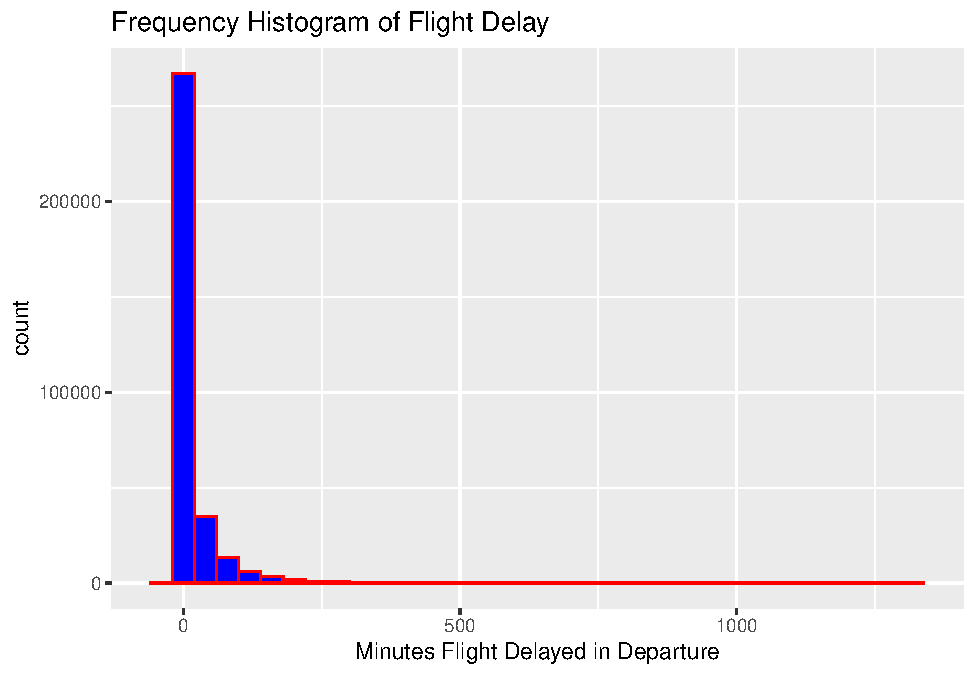
\includegraphics{A4_files/figure-latex/unnamed-chunk-5-1.pdf} \textbf{b}
The statistical hypothesis to be tested is

\[
\begin{eqnarray}
{\rm H}_{0}: \text{the race of the victim does Not appear to affect whether an African-American convicted of murder in Georgia will receive a death sentence} \\
{\rm H}_{A}: \text{the race of the victim does appear to affect whether an African-American convicted of murder in Georgia will receive a death sentence} \\
\end{eqnarray}
\] I set up the \(\alpha = 0.05\)

\begin{Shaded}
\begin{Highlighting}[]
\NormalTok{death }\OtherTok{=} \FunctionTok{rbind}\NormalTok{(}\FunctionTok{c}\NormalTok{(}\DecValTok{45}\NormalTok{,}\DecValTok{85}\NormalTok{), }\FunctionTok{c}\NormalTok{(}\DecValTok{14}\NormalTok{, }\DecValTok{218}\NormalTok{))}
\FunctionTok{rownames}\NormalTok{(death) }\OtherTok{=} \FunctionTok{c}\NormalTok{(}\StringTok{"Victim was Caucasian"}\NormalTok{, }\StringTok{"Victim was African{-}American"}\NormalTok{)}
\FunctionTok{colnames}\NormalTok{(death) }\OtherTok{=} \FunctionTok{c}\NormalTok{(}\StringTok{"Sentenced to Death"}\NormalTok{, }\StringTok{"Not Sentenced to Death"}\NormalTok{)}
\NormalTok{death}
\end{Highlighting}
\end{Shaded}

\begin{verbatim}
##                             Sentenced to Death Not Sentenced to Death
## Victim was Caucasian                        45                     85
## Victim was African-American                 14                    218
\end{verbatim}

\begin{Shaded}
\begin{Highlighting}[]
\FunctionTok{chisq.test}\NormalTok{(death, }\AttributeTok{correct=}\ConstantTok{FALSE}\NormalTok{)}
\end{Highlighting}
\end{Shaded}

\begin{verbatim}
## 
##  Pearson's Chi-squared test
## 
## data:  death
## X-squared = 49.888, df = 1, p-value = 1.628e-12
\end{verbatim}

\begin{Shaded}
\begin{Highlighting}[]
\NormalTok{pvalue }\OtherTok{=} \FloatTok{1.628e{-}12}
\NormalTok{pvalue}
\end{Highlighting}
\end{Shaded}

\begin{verbatim}
## [1] 1.628e-12
\end{verbatim}

Because \(p-value < \alpha\), Reject \(H_{0}\). I conclude that the race
of the victim does appear to affect whether an African-American
convicted of murder in Georgia will receive a death sentence.

The confidence interval:

\begin{Shaded}
\begin{Highlighting}[]
\FunctionTok{prop.test}\NormalTok{(}\FunctionTok{c}\NormalTok{(}\DecValTok{45}\NormalTok{,}\DecValTok{14}\NormalTok{), }\FunctionTok{c}\NormalTok{(}\DecValTok{45}\SpecialCharTok{+}\DecValTok{85}\NormalTok{,}\DecValTok{14}\SpecialCharTok{+}\DecValTok{218}\NormalTok{), }\AttributeTok{alternative=}\StringTok{"two.sided"}\NormalTok{, }\AttributeTok{correct=}\ConstantTok{FALSE}\NormalTok{)}
\end{Highlighting}
\end{Shaded}

\begin{verbatim}
## 
##  2-sample test for equality of proportions without continuity
##  correction
## 
## data:  c out of c45 out of 45 + 8514 out of 14 + 218
## X-squared = 49.888, df = 1, p-value = 1.628e-12
## alternative hypothesis: two.sided
## 95 percent confidence interval:
##  0.1984768 0.3731412
## sample estimates:
##     prop 1     prop 2 
## 0.34615385 0.06034483
\end{verbatim}

The 95 percent confidence interval is: (0.1984768, 0.3731412)

\hypertarget{q3}{%
\subsection{Q3}\label{q3}}

\textbf{a}

\begin{Shaded}
\begin{Highlighting}[]
\NormalTok{df.q3 }\OtherTok{=} \FunctionTok{read.csv}\NormalTok{(}\StringTok{"http://people.ucalgary.ca/\textasciitilde{}jbstall/DataFiles/CloudSeedingData.csv"}\NormalTok{)}
\FunctionTok{head}\NormalTok{(df.q3)}
\end{Highlighting}
\end{Shaded}

\begin{verbatim}
##   RAINFALL TREATMENT
## 1   1202.6  UNSEEDED
## 2    830.1  UNSEEDED
## 3    372.4  UNSEEDED
## 4    345.5  UNSEEDED
## 5    321.2  UNSEEDED
## 6    244.3  UNSEEDED
\end{verbatim}

\begin{Shaded}
\begin{Highlighting}[]
\FunctionTok{tail}\NormalTok{(df.q3)}
\end{Highlighting}
\end{Shaded}

\begin{verbatim}
##    RAINFALL TREATMENT
## 47     40.6    SEEDED
## 48     32.7    SEEDED
## 49     31.4    SEEDED
## 50     17.5    SEEDED
## 51      7.7    SEEDED
## 52      4.1    SEEDED
\end{verbatim}

\[
\hspace{0.25in} {\rm H}_{0}: \mu_{seeded} - \mu_{unseeded} = 0 \hspace{0.25in} \text{(cloud seeding does not have an effect on rainfall on average)}
\\
\hspace{0.25in} {\rm H}_{A}: \mu_{seeded} - \mu_{unseeded} \ne 0 \hspace{0.25in} \text{(cloud seeding does have an effect on rainfall on average)}
\] I set up the \(\alpha = 0.05\)

\begin{Shaded}
\begin{Highlighting}[]
\FunctionTok{t.test}\NormalTok{(}\SpecialCharTok{\textasciitilde{}}\NormalTok{RAINFALL}\SpecialCharTok{|}\NormalTok{TREATMENT, }\AttributeTok{conf.level=}\FloatTok{0.95}\NormalTok{, }\AttributeTok{alternative =} \StringTok{"two.sided"}\NormalTok{, }\AttributeTok{var.equal=}\ConstantTok{FALSE}\NormalTok{, df.q3)}
\end{Highlighting}
\end{Shaded}

\begin{verbatim}
## 
##  Welch Two Sample t-test
## 
## data:  RAINFALL by TREATMENT
## t = 1.9982, df = 33.855, p-value = 0.05377
## alternative hypothesis: true difference in means between group SEEDED and group UNSEEDED is not equal to 0
## 95 percent confidence interval:
##   -4.764295 559.556603
## sample estimates:
##   mean in group SEEDED mean in group UNSEEDED 
##               441.9846               164.5885
\end{verbatim}

Because \(p-value > \alpha\), Fail to Reject \(H_{0}\). I conclude that,
on average, cloud seeding does not have an effect on rainfall. The 95
percent confidence interval is: (-4.764295, 559.556603)

\begin{Shaded}
\begin{Highlighting}[]
\NormalTok{n.SEEDED }\OtherTok{=} \FunctionTok{favstats}\NormalTok{(}\SpecialCharTok{\textasciitilde{}}\NormalTok{RAINFALL}\SpecialCharTok{|}\NormalTok{TREATMENT, }\AttributeTok{data=}\NormalTok{df.q3)}\SpecialCharTok{$}\NormalTok{n[}\DecValTok{1}\NormalTok{] }
\NormalTok{n.UNSEEDED }\OtherTok{=} \FunctionTok{favstats}\NormalTok{(}\SpecialCharTok{\textasciitilde{}}\NormalTok{RAINFALL}\SpecialCharTok{|}\NormalTok{TREATMENT, }\AttributeTok{data=}\NormalTok{df.q3)}\SpecialCharTok{$}\NormalTok{n[}\DecValTok{2}\NormalTok{]}
\NormalTok{n.SEEDED}
\end{Highlighting}
\end{Shaded}

\begin{verbatim}
## [1] 26
\end{verbatim}

\begin{Shaded}
\begin{Highlighting}[]
\NormalTok{n.UNSEEDED}
\end{Highlighting}
\end{Shaded}

\begin{verbatim}
## [1] 26
\end{verbatim}

\begin{Shaded}
\begin{Highlighting}[]
\CommentTok{\#n \textgreater{} 25 }
\CommentTok{\#Condition satisfied}
\end{Highlighting}
\end{Shaded}

\textbf{b} \[
\hspace{0.25in} {\rm H}_{0}: \frac{\sigma_{seeded}}{\sigma_{unseeded}} \ge 1 \hspace{0.25in} 
\\
\hspace{0.25in} {\rm H}_{A}: \frac{\sigma_{seeded}}{\sigma_{unseeded}} < 1  
\] I set up the \(\alpha = 0.05\)

\begin{Shaded}
\begin{Highlighting}[]
\FunctionTok{favstats}\NormalTok{(}\SpecialCharTok{\textasciitilde{}}\NormalTok{RAINFALL}\SpecialCharTok{|}\NormalTok{TREATMENT, }\AttributeTok{data=}\NormalTok{df.q3)}
\end{Highlighting}
\end{Shaded}

\begin{verbatim}
##   TREATMENT min     Q1 median      Q3    max     mean       sd  n missing
## 1    SEEDED 4.1 98.125  221.6 406.025 2745.6 441.9846 650.7872 26       0
## 2  UNSEEDED 1.0 24.825   44.2 159.200 1202.6 164.5885 278.4264 26       0
\end{verbatim}

\begin{Shaded}
\begin{Highlighting}[]
\FunctionTok{favstats}\NormalTok{(}\SpecialCharTok{\textasciitilde{}}\NormalTok{RAINFALL}\SpecialCharTok{|}\NormalTok{TREATMENT, }\AttributeTok{data=}\NormalTok{df.q3)}\SpecialCharTok{$}\NormalTok{sd[}\DecValTok{2}\NormalTok{]}
\end{Highlighting}
\end{Shaded}

\begin{verbatim}
## [1] 278.4264
\end{verbatim}

\begin{Shaded}
\begin{Highlighting}[]
\FunctionTok{favstats}\NormalTok{(}\SpecialCharTok{\textasciitilde{}}\NormalTok{RAINFALL}\SpecialCharTok{|}\NormalTok{TREATMENT, }\AttributeTok{data=}\NormalTok{df.q3)}\SpecialCharTok{$}\NormalTok{sd[}\DecValTok{1}\NormalTok{] }\SpecialCharTok{/} \FunctionTok{favstats}\NormalTok{(}\SpecialCharTok{\textasciitilde{}}\NormalTok{RAINFALL}\SpecialCharTok{|}\NormalTok{TREATMENT, }\AttributeTok{data=}\NormalTok{df.q3)}\SpecialCharTok{$}\NormalTok{sd[}\DecValTok{2}\NormalTok{]}
\end{Highlighting}
\end{Shaded}

\begin{verbatim}
## [1] 2.337376
\end{verbatim}

\begin{Shaded}
\begin{Highlighting}[]
\NormalTok{sd.obs }\OtherTok{=} \FunctionTok{favstats}\NormalTok{(}\SpecialCharTok{\textasciitilde{}}\NormalTok{RAINFALL}\SpecialCharTok{|}\NormalTok{TREATMENT, }\AttributeTok{data=}\NormalTok{df.q3)}\SpecialCharTok{$}\NormalTok{sd[}\DecValTok{1}\NormalTok{] }\SpecialCharTok{/} \FunctionTok{favstats}\NormalTok{(}\SpecialCharTok{\textasciitilde{}}\NormalTok{RAINFALL}\SpecialCharTok{|}\NormalTok{TREATMENT, }\AttributeTok{data=}\NormalTok{df.q3)}\SpecialCharTok{$}\NormalTok{sd[}\DecValTok{2}\NormalTok{]}

\NormalTok{outcome }\OtherTok{=} \FunctionTok{numeric}\NormalTok{(}\DecValTok{2000}\NormalTok{) }\CommentTok{\#create a vector to store rate of sd}
\ControlFlowTok{for}\NormalTok{(i }\ControlFlowTok{in} \DecValTok{1}\SpecialCharTok{:}\DecValTok{2000}\NormalTok{)}
\NormalTok{\{ index }\OtherTok{=} \FunctionTok{sample}\NormalTok{(}\DecValTok{52}\NormalTok{, }\DecValTok{26}\NormalTok{, }\AttributeTok{replace=}\ConstantTok{FALSE}\NormalTok{)  }
\NormalTok{  outcome[i] }\OtherTok{=} \FunctionTok{sd}\NormalTok{(df.q3}\SpecialCharTok{$}\NormalTok{RAINFALL[index]) }\SpecialCharTok{/} \FunctionTok{sd}\NormalTok{(df.q3}\SpecialCharTok{$}\NormalTok{RAINFALL[}\SpecialCharTok{{-}}\NormalTok{index]) }
\NormalTok{\}}
\FunctionTok{hist}\NormalTok{(outcome, }\AttributeTok{xlab=}\StringTok{"Rate of Sd"}\NormalTok{, }\AttributeTok{ylab=}\StringTok{"Frequency"}\NormalTok{, }\AttributeTok{main=}\StringTok{"Outcome of 2000 Permutation Tests"}\NormalTok{, }\AttributeTok{col=}\StringTok{\textquotesingle{}blue\textquotesingle{}}\NormalTok{)}
\FunctionTok{abline}\NormalTok{(}\AttributeTok{v =}\NormalTok{ sd.obs, }\AttributeTok{col=}\StringTok{"red"}\NormalTok{)}
\end{Highlighting}
\end{Shaded}

\includegraphics{A4_files/figure-latex/unnamed-chunk-12-1.pdf}

\begin{Shaded}
\begin{Highlighting}[]
\NormalTok{pvalueq3b }\OtherTok{=}\NormalTok{ (}\FunctionTok{sum}\NormalTok{(outcome }\SpecialCharTok{\textless{}=}\NormalTok{ sd.obs) )}\SpecialCharTok{/}\NormalTok{(}\DecValTok{2000}\NormalTok{)  }\CommentTok{\#computes P{-}value}
\NormalTok{pvalueq3b}
\end{Highlighting}
\end{Shaded}

\begin{verbatim}
## [1] 0.9315
\end{verbatim}

Because \(p-value > \alpha\), Fail to Reject \(H_{0}\).

\textbf{c}

\begin{Shaded}
\begin{Highlighting}[]
\NormalTok{df.q3 }\OtherTok{=}\NormalTok{ df.q3 }\SpecialCharTok{\%\textgreater{}\%}
  \FunctionTok{mutate}\NormalTok{(}\AttributeTok{Ln =} \FunctionTok{log}\NormalTok{(RAINFALL)) }\CommentTok{\#create a new variable called Diff = price of camera at JR {-} price of same camera at BH}
\FunctionTok{head}\NormalTok{(df.q3)}
\end{Highlighting}
\end{Shaded}

\begin{verbatim}
##   RAINFALL TREATMENT       Ln
## 1   1202.6  UNSEEDED 7.092241
## 2    830.1  UNSEEDED 6.721546
## 3    372.4  UNSEEDED 5.919969
## 4    345.5  UNSEEDED 5.844993
## 5    321.2  UNSEEDED 5.772064
## 6    244.3  UNSEEDED 5.498397
\end{verbatim}

\[
\hspace{0.25in}  {\rm H}_{0}: \overline{ln(X_{SEEDED})} - \widetilde{ln(X_{UNSEEDED})} = 0 \hspace{0.25in} 
\\
\hspace{0.25in} {\rm H}_{A}: \overline{ln(X_{SEEDED})} - \widetilde{ln(X_{UNSEEDED})} \neq 0 \hspace{0.25in} 
\] I set up the \(\alpha = 0.05\)

\begin{Shaded}
\begin{Highlighting}[]
\FunctionTok{favstats}\NormalTok{(}\SpecialCharTok{\textasciitilde{}}\NormalTok{RAINFALL}\SpecialCharTok{|}\NormalTok{TREATMENT, }\AttributeTok{data=}\NormalTok{df.q3)}
\end{Highlighting}
\end{Shaded}

\begin{verbatim}
##   TREATMENT min     Q1 median      Q3    max     mean       sd  n missing
## 1    SEEDED 4.1 98.125  221.6 406.025 2745.6 441.9846 650.7872 26       0
## 2  UNSEEDED 1.0 24.825   44.2 159.200 1202.6 164.5885 278.4264 26       0
\end{verbatim}

\begin{Shaded}
\begin{Highlighting}[]
\NormalTok{diffmd.obs }\OtherTok{=} \FunctionTok{favstats}\NormalTok{(}\SpecialCharTok{\textasciitilde{}}\NormalTok{Ln}\SpecialCharTok{|}\NormalTok{TREATMENT, }\AttributeTok{data=}\NormalTok{df.q3)}\SpecialCharTok{$}\NormalTok{mean[}\DecValTok{1}\NormalTok{] }\SpecialCharTok{{-}} \FunctionTok{favstats}\NormalTok{(}\SpecialCharTok{\textasciitilde{}}\NormalTok{Ln}\SpecialCharTok{|}\NormalTok{TREATMENT, }\AttributeTok{data=}\NormalTok{df.q3)}\SpecialCharTok{$}\NormalTok{median[}\DecValTok{2}\NormalTok{]}

\NormalTok{outcome3c }\OtherTok{=} \FunctionTok{numeric}\NormalTok{(}\DecValTok{2000}\NormalTok{) }\CommentTok{\#create a vector to store}
\ControlFlowTok{for}\NormalTok{(i }\ControlFlowTok{in} \DecValTok{1}\SpecialCharTok{:}\DecValTok{2000}\NormalTok{)}
\NormalTok{\{ index }\OtherTok{=} \FunctionTok{sample}\NormalTok{(}\DecValTok{52}\NormalTok{, }\DecValTok{26}\NormalTok{, }\AttributeTok{replace=}\ConstantTok{FALSE}\NormalTok{)  }
\NormalTok{  outcome3c[i] }\OtherTok{=} \FunctionTok{mean}\NormalTok{(df.q3}\SpecialCharTok{$}\NormalTok{Ln[index]) }\SpecialCharTok{{-}} \FunctionTok{median}\NormalTok{(df.q3}\SpecialCharTok{$}\NormalTok{Ln[}\SpecialCharTok{{-}}\NormalTok{index]) }
\NormalTok{\}}
\FunctionTok{hist}\NormalTok{(outcome3c, }\AttributeTok{xlab=}\StringTok{"Diff of Median ln"}\NormalTok{, }\AttributeTok{ylab=}\StringTok{"Frequency"}\NormalTok{, }\AttributeTok{main=}\StringTok{"Outcome of 2000 Permutation Tests"}\NormalTok{, }\AttributeTok{col=}\StringTok{\textquotesingle{}blue\textquotesingle{}}\NormalTok{)}
\FunctionTok{abline}\NormalTok{(}\AttributeTok{v =}\NormalTok{ diffmd.obs, }\AttributeTok{col=}\StringTok{"red"}\NormalTok{)}
\end{Highlighting}
\end{Shaded}

\includegraphics{A4_files/figure-latex/unnamed-chunk-15-1.pdf}

\begin{Shaded}
\begin{Highlighting}[]
\NormalTok{pvalueq3 }\OtherTok{=}\NormalTok{ (}\FunctionTok{sum}\NormalTok{(outcome3c }\SpecialCharTok{\textgreater{}=}\NormalTok{ diffmd.obs) }\SpecialCharTok{+} \FunctionTok{sum}\NormalTok{(outcome3c }\SpecialCharTok{\textless{}=}  \SpecialCharTok{{-}}\NormalTok{diffmd.obs))}\SpecialCharTok{/}\NormalTok{(}\DecValTok{2000}\NormalTok{)  }\CommentTok{\#computes P{-}value}
\NormalTok{pvalueq3}
\end{Highlighting}
\end{Shaded}

\begin{verbatim}
## [1] 0.018
\end{verbatim}

Because \(p-value < \alpha\),Reject \(H_{0}\).

\begin{Shaded}
\begin{Highlighting}[]
\FunctionTok{favstats}\NormalTok{(outcome3c)}
\end{Highlighting}
\end{Shaded}

\begin{verbatim}
##        min         Q1     median        Q3     max       mean        sd    n
##  -1.730198 -0.5040246 -0.1848319 0.1428779 1.78175 -0.1748081 0.5280139 2000
##  missing
##        0
\end{verbatim}

\begin{Shaded}
\begin{Highlighting}[]
\NormalTok{diffmd.obs}
\end{Highlighting}
\end{Shaded}

\begin{verbatim}
## [1] 1.347928
\end{verbatim}

\#\#Q4

The statistical hypothesis to be tested is

\[
\begin{eqnarray}
{\rm H}_{0}: p_{minoxidil} & \leq  & p_{placebo} \hspace{0.2in} \text{(minoxidil is not effective in treating male pattern baldness )} \\
{\rm H}_{A}: p_{minoxidil} & >  & p_{placebo} \text{(minoxidil is effective in treating male pattern baldness )} \\
\end{eqnarray}
\] If the Vitamin C is more effective then:

\[
\begin{eqnarray}
p_{minoxidil} > p_{Placebo} \longrightarrow p_{minoxidil} - p_{Placebo} > 0
\end{eqnarray}
\]

I set up the \(\alpha = 0.05\)

\begin{Shaded}
\begin{Highlighting}[]
\FunctionTok{prop.test}\NormalTok{(}\FunctionTok{c}\NormalTok{(}\DecValTok{99}\NormalTok{,}\DecValTok{62}\NormalTok{), }\FunctionTok{c}\NormalTok{(}\DecValTok{310}\NormalTok{,}\DecValTok{309}\NormalTok{), }\AttributeTok{alternative=}\StringTok{"greater"}\NormalTok{, }\AttributeTok{correct=}\ConstantTok{FALSE}\NormalTok{)}
\end{Highlighting}
\end{Shaded}

\begin{verbatim}
## 
##  2-sample test for equality of proportions without continuity
##  correction
## 
## data:  c out of c99 out of 31062 out of 309
## X-squared = 11.331, df = 1, p-value = 0.0003811
## alternative hypothesis: greater
## 95 percent confidence interval:
##  0.06124968 1.00000000
## sample estimates:
##    prop 1    prop 2 
## 0.3193548 0.2006472
\end{verbatim}

Because \(p-value < \alpha\), Reject
\(H_{0}:p_{minoxidil} \le p_{placebo}\). I conclude that minoxidil is
effective in treating male pattern baldness.

95 percent confidence interval is from 0.06124968 to 1.

In the context of these data, the p-value is the probability that , in
another experimental study like this, the\$ p\_\{minoxidil\} -
p\_\{Placebo\}\$ will be smaller than test statistic we have this time,
assuming that the null hypothesis is true. In this case, p value is
0.0003811, which means the above statement is not likely to happen.

\hypertarget{q5}{%
\subsection{Q5}\label{q5}}

\textbf{a}

\begin{Shaded}
\begin{Highlighting}[]
\NormalTok{df.q5 }\OtherTok{=} \FunctionTok{read.csv}\NormalTok{(}\StringTok{"http://people.ucalgary.ca/\textasciitilde{}jbstall/DataFiles/chocnochocratings.csv"}\NormalTok{)}
\NormalTok{df.q5}
\end{Highlighting}
\end{Shaded}

\begin{verbatim}
##    Particpant Class Group GroupName Q9 Overall
## 1           1     1     1 Chocolate  3    2.44
## 2           2     1     1 Chocolate  3    2.56
## 3           3     1     1 Chocolate  5    4.33
## 4           4     1     1 Chocolate  4    4.56
## 5           5     1     1 Chocolate  5    4.56
## 6           6     1     1 Chocolate  5    4.22
## 7           7     1     1 Chocolate  3    3.56
## 8           8     1     1 Chocolate  5    4.67
## 9           9     1     1 Chocolate  4    3.67
## 10         10     1     1 Chocolate  4    4.22
## 11         11     1     1 Chocolate  2    2.67
## 12         12     1     1 Chocolate  4    4.11
## 13         13     1     1 Chocolate  5    4.89
## 14         14     1     1 Chocolate  4    4.22
## 15         15     1     1 Chocolate  4    3.89
## 16         16     1     1 Chocolate  4    3.78
## 17         17     1     1 Chocolate  3    2.89
## 18         18     1     2    NOChoc  4    3.67
## 19         19     1     2    NOChoc  3    2.56
## 20         20     1     2    NOChoc  3    3.33
## 21         21     1     2    NOChoc  4    3.44
## 22         22     1     2    NOChoc  3    2.89
## 23         23     1     2    NOChoc  4    3.78
## 24         24     1     2    NOChoc  5    5.00
## 25         25     1     2    NOChoc  5    4.44
## 26         26     1     2    NOChoc  4    3.67
## 27         27     1     2    NOChoc  3    3.00
## 28         28     1     2    NOChoc  1    2.00
## 29         29     1     2    NOChoc  4    3.78
## 30         30     2     1 Chocolate  5    4.44
## 31         31     2     1 Chocolate  5    4.56
## 32         32     2     1 Chocolate  5    4.78
## 33         33     2     1 Chocolate  3    3.44
## 34         34     2     1 Chocolate  3    3.67
## 35         35     2     1 Chocolate  4    4.00
## 36         36     2     1 Chocolate  4    4.00
## 37         37     2     1 Chocolate  5    4.11
## 38         38     2     1 Chocolate  5    5.00
## 39         39     2     1 Chocolate  3    3.67
## 40         40     2     1 Chocolate  3    3.67
## 41         41     2     1 Chocolate  2    3.00
## 42         42     2     1 Chocolate  5    4.56
## 43         43     2     1 Chocolate  4    4.00
## 44         44     2     1 Chocolate  4    4.11
## 45         45     2     2    NOChoc  4    3.33
## 46         46     2     2    NOChoc  3    3.11
## 47         47     2     2    NOChoc  4    3.89
## 48         48     2     2    NOChoc  5    4.22
## 49         49     2     2    NOChoc  4    4.22
## 50         50     2     2    NOChoc  5    5.00
## 51         51     2     2    NOChoc  4    4.22
## 52         52     2     2    NOChoc  5    3.89
## 53         53     2     2    NOChoc  3    2.78
## 54         54     2     2    NOChoc  5    4.67
## 55         55     2     2    NOChoc  5    3.89
## 56         56     2     2    NOChoc  4    3.89
## 57         57     2     2    NOChoc  5    4.22
## 58         58     2     2    NOChoc  4    4.00
## 59         59     2     2    NOChoc  4    3.78
## 60         60     2     2    NOChoc  4    4.00
## 61         61     2     2    NOChoc  3    3.56
## 62         62     2     2    NOChoc  4    4.00
## 63         63     2     2    NOChoc  2    3.11
## 64         64     3     1 Chocolate  5    4.44
## 65         65     3     1 Chocolate  3    2.89
## 66         66     3     1 Chocolate  5    4.89
## 67         67     3     1 Chocolate  5    4.89
## 68         68     3     1 Chocolate  5    4.56
## 69         69     3     1 Chocolate  5    5.00
## 70         70     3     1 Chocolate  4    4.56
## 71         71     3     1 Chocolate  5    4.67
## 72         72     3     1 Chocolate  5    4.67
## 73         73     3     1 Chocolate  5    5.00
## 74         74     3     1 Chocolate  5    5.00
## 75         75     3     1 Chocolate  3    3.67
## 76         76     3     1 Chocolate  3    3.00
## 77         77     3     1 Chocolate  5    4.44
## 78         78     3     1 Chocolate  4    3.89
## 79         79     3     1 Chocolate  3    3.67
## 80         80     3     1 Chocolate  4    3.78
## 81         81     3     1 Chocolate  5    4.33
## 82         82     3     2    NOChoc  3    4.33
## 83         83     3     2    NOChoc  5    4.44
## 84         84     3     2    NOChoc  3    3.00
## 85         85     3     2    NOChoc  3    3.56
## 86         86     3     2    NOChoc  4    4.22
## 87         87     3     2    NOChoc  3    3.89
## 88         88     3     2    NOChoc  4    4.22
## 89         89     3     2    NOChoc  5    4.56
## 90         90     3     2    NOChoc  3    3.78
## 91         91     3     2    NOChoc  4    4.22
## 92         92     3     2    NOChoc  3    3.00
## 93         93     3     2    NOChoc  5    4.67
## 94         94     3     2    NOChoc  4    4.22
## 95         95     3     2    NOChoc  5    4.56
## 96         96     3     2    NOChoc  5    4.33
## 97         97     3     2    NOChoc  5    4.56
## 98         98     3     2    NOChoc  4    3.89
\end{verbatim}

Treatment effect means that student who got chocolate rate prof. higher
than student who did not receive chocolate.

The statistical hypothesis to be tested is

\[
\begin{eqnarray}
{\rm H}_{0}: \mu_{ChocolateQ9} & \leq  & \mu_{NOChocQ9} \hspace{0.2in} \text{(there is not a treatment effect)} \\
{\rm H}_{A}: \mu_{ChocolateQ9} & >  & \mu_{NOChocQ9} \hspace{0.2in} \text{(there is a treatment effect)} \\
\end{eqnarray}
\] If Treatment effect is true then: \[
\mu_{ChocolateQ9} > \mu_{NOChocQ9} \longrightarrow \mu_{ChocolateQ9} - \mu_{NOChocQ9} > 0
\]

I set up the \(\alpha = 0.05\)

\begin{Shaded}
\begin{Highlighting}[]
\FunctionTok{favstats}\NormalTok{(}\SpecialCharTok{\textasciitilde{}}\NormalTok{Q9}\SpecialCharTok{|}\NormalTok{GroupName, }\AttributeTok{data=}\NormalTok{df.q5)}
\end{Highlighting}
\end{Shaded}

\begin{verbatim}
##   GroupName min Q1 median Q3 max     mean        sd  n missing
## 1 Chocolate   2  3      4  5   5 4.120000 0.9178502 50       0
## 2    NOChoc   1  3      4  5   5 3.916667 0.9186793 48       0
\end{verbatim}

\begin{Shaded}
\begin{Highlighting}[]
\FunctionTok{favstats}\NormalTok{(}\SpecialCharTok{\textasciitilde{}}\NormalTok{Q9}\SpecialCharTok{|}\NormalTok{GroupName, }\AttributeTok{data=}\NormalTok{df.q5)}\SpecialCharTok{$}\NormalTok{mean[}\DecValTok{1}\NormalTok{]}
\end{Highlighting}
\end{Shaded}

\begin{verbatim}
## [1] 4.12
\end{verbatim}

\begin{Shaded}
\begin{Highlighting}[]
\FunctionTok{favstats}\NormalTok{(}\SpecialCharTok{\textasciitilde{}}\NormalTok{Q9}\SpecialCharTok{|}\NormalTok{GroupName, }\AttributeTok{data=}\NormalTok{df.q5)}\SpecialCharTok{$}\NormalTok{mean[}\DecValTok{2}\NormalTok{]}
\end{Highlighting}
\end{Shaded}

\begin{verbatim}
## [1] 3.916667
\end{verbatim}

\begin{Shaded}
\begin{Highlighting}[]
\FunctionTok{favstats}\NormalTok{(}\SpecialCharTok{\textasciitilde{}}\NormalTok{Q9}\SpecialCharTok{|}\NormalTok{GroupName, }\AttributeTok{data=}\NormalTok{df.q5)}\SpecialCharTok{$}\NormalTok{n[}\DecValTok{1}\NormalTok{]}
\end{Highlighting}
\end{Shaded}

\begin{verbatim}
## [1] 50
\end{verbatim}

\begin{Shaded}
\begin{Highlighting}[]
\FunctionTok{favstats}\NormalTok{(}\SpecialCharTok{\textasciitilde{}}\NormalTok{Q9}\SpecialCharTok{|}\NormalTok{GroupName, }\AttributeTok{data=}\NormalTok{df.q5)}\SpecialCharTok{$}\NormalTok{n[}\DecValTok{2}\NormalTok{]}
\end{Highlighting}
\end{Shaded}

\begin{verbatim}
## [1] 48
\end{verbatim}

\begin{Shaded}
\begin{Highlighting}[]
\NormalTok{n }\OtherTok{=} \FunctionTok{favstats}\NormalTok{(}\SpecialCharTok{\textasciitilde{}}\NormalTok{Q9}\SpecialCharTok{|}\NormalTok{GroupName, }\AttributeTok{data=}\NormalTok{df.q5)}\SpecialCharTok{$}\NormalTok{n[}\DecValTok{1}\NormalTok{] }\SpecialCharTok{+} \FunctionTok{favstats}\NormalTok{(}\SpecialCharTok{\textasciitilde{}}\NormalTok{Q9}\SpecialCharTok{|}\NormalTok{GroupName, }\AttributeTok{data=}\NormalTok{df.q5)}\SpecialCharTok{$}\NormalTok{n[}\DecValTok{2}\NormalTok{]}
\NormalTok{n}
\end{Highlighting}
\end{Shaded}

\begin{verbatim}
## [1] 98
\end{verbatim}

\begin{Shaded}
\begin{Highlighting}[]
\CommentTok{\#1 cho}
\CommentTok{\#2 nocho}
\end{Highlighting}
\end{Shaded}

\begin{Shaded}
\begin{Highlighting}[]
\NormalTok{obsdiff5 }\OtherTok{=} \FunctionTok{favstats}\NormalTok{(}\SpecialCharTok{\textasciitilde{}}\NormalTok{Q9}\SpecialCharTok{|}\NormalTok{GroupName, }\AttributeTok{data=}\NormalTok{df.q5)}\SpecialCharTok{$}\NormalTok{mean[}\DecValTok{1}\NormalTok{] }\SpecialCharTok{{-}} \FunctionTok{favstats}\NormalTok{(}\SpecialCharTok{\textasciitilde{}}\NormalTok{Q9}\SpecialCharTok{|}\NormalTok{GroupName, }\AttributeTok{data=}\NormalTok{df.q5)}\SpecialCharTok{$}\NormalTok{mean[}\DecValTok{2}\NormalTok{]}
\NormalTok{N }\OtherTok{=}\DecValTok{2000}
\NormalTok{outcome5 }\OtherTok{=} \FunctionTok{numeric}\NormalTok{(N)}
\ControlFlowTok{for}\NormalTok{ (i }\ControlFlowTok{in} \DecValTok{1}\SpecialCharTok{:}\NormalTok{N)\{}
\NormalTok{  index }\OtherTok{=} \FunctionTok{sample}\NormalTok{(}\DecValTok{98}\NormalTok{, }\DecValTok{50}\NormalTok{, }\AttributeTok{replace =} \ConstantTok{FALSE}\NormalTok{)}
\NormalTok{  outcome5[i] }\OtherTok{=} \FunctionTok{mean}\NormalTok{(df.q5}\SpecialCharTok{$}\NormalTok{Q9[index]) }\SpecialCharTok{{-}} \FunctionTok{mean}\NormalTok{(df.q5}\SpecialCharTok{$}\NormalTok{Q9[}\SpecialCharTok{{-}}\NormalTok{index])}
\NormalTok{\}}

\FunctionTok{hist}\NormalTok{(outcome5, }\AttributeTok{xlab=}\StringTok{"Difference Between Mean rate point of Chocolate and Mean rate point of NOChoc"}\NormalTok{, }\AttributeTok{ylab=}\StringTok{"Frequency"}\NormalTok{, }\AttributeTok{main=}\StringTok{"Outcome of 2000 Permutation Tests"}\NormalTok{, }\AttributeTok{col=}\StringTok{\textquotesingle{}blue\textquotesingle{}}\NormalTok{)}
\FunctionTok{abline}\NormalTok{(}\AttributeTok{v =}\NormalTok{ obsdiff5, }\AttributeTok{col=}\StringTok{"red"}\NormalTok{)}
\end{Highlighting}
\end{Shaded}

\includegraphics{A4_files/figure-latex/unnamed-chunk-20-1.pdf}

\begin{Shaded}
\begin{Highlighting}[]
\NormalTok{pvalueq5 }\OtherTok{=}\NormalTok{ (}\FunctionTok{sum}\NormalTok{(outcome5 }\SpecialCharTok{\textgreater{}=}\NormalTok{ obsdiff5))}\SpecialCharTok{/}\NormalTok{(N)  }\CommentTok{\#computes P{-}value}
\NormalTok{pvalueq5}
\end{Highlighting}
\end{Shaded}

\begin{verbatim}
## [1] 0.16
\end{verbatim}

Because \(p-value > \alpha\), Fail to Reject \(H_{0}\). I conclude that
there is not a treatment effect which means that student who got
chocolate did not rate prof. higher than student who did not receive
chocolate in Q9 on average.

\textbf{b} The statistical hypothesis to be tested is

\[
\begin{eqnarray}
{\rm H}_{0}: \mu_{ChocolateOverall} & \leq  & \mu_{NOChocOverall} \hspace{0.2in} \text{(there is not a treatment effect)} \\
{\rm H}_{A}: \mu_{ChocolateOverall} & >  & \mu_{NOChocOverall} \hspace{0.2in} \text{(there is a treatment effect)} \\
\end{eqnarray}
\]

\(n > 25\) Condition satisfied I set up the \(\alpha = 0.05\)

\begin{Shaded}
\begin{Highlighting}[]
\FunctionTok{t.test}\NormalTok{(}\SpecialCharTok{\textasciitilde{}}\NormalTok{Overall}\SpecialCharTok{|}\NormalTok{GroupName, }\AttributeTok{alternative =} \StringTok{"greater"}\NormalTok{, }\AttributeTok{conf.level=}\FloatTok{0.95}\NormalTok{, }\AttributeTok{var.equal=}\ConstantTok{FALSE}\NormalTok{, df.q5)}
\end{Highlighting}
\end{Shaded}

\begin{verbatim}
## 
##  Welch Two Sample t-test
## 
## data:  Overall by GroupName
## t = 1.6616, df = 95.93, p-value = 0.04993
## alternative hypothesis: true difference in means between group Chocolate and group NOChoc is greater than 0
## 95 percent confidence interval:
##  9.400666e-05          Inf
## sample estimates:
## mean in group Chocolate    mean in group NOChoc 
##                4.072000                3.849792
\end{verbatim}

Because \(p-value < \alpha\), Reject \(H_{0}\).

I conclude that there is a treatment effect which means that student who
got chocolate did not rate prof. higher than student who did not receive
chocolate in Overall on average. In the context of these data, the
p-value is the probability that , in another experimental study like
this, the\(\mu_{ChocolateOverall} - \mu_{NOChocOverall}\) will be larger
than test statistic we have this time, assuming that the null hypothesis
is true.

\textbf{c}

\begin{Shaded}
\begin{Highlighting}[]
\FunctionTok{ggplot}\NormalTok{(}\FunctionTok{filter}\NormalTok{(df.q5, GroupName }\SpecialCharTok{==}\StringTok{"Chocolate"}\NormalTok{), }\FunctionTok{aes}\NormalTok{(}\AttributeTok{sample =}\NormalTok{ Q9)) }\SpecialCharTok{+} \FunctionTok{stat\_qq}\NormalTok{(}\AttributeTok{col=}\StringTok{"blue"}\NormalTok{) }\SpecialCharTok{+} \FunctionTok{stat\_qqline}\NormalTok{(}\AttributeTok{col=}\StringTok{"red"}\NormalTok{) }\SpecialCharTok{+} \FunctionTok{ggtitle}\NormalTok{(}\StringTok{"Normal Probability Plot"}\NormalTok{)}
\end{Highlighting}
\end{Shaded}

\includegraphics{A4_files/figure-latex/unnamed-chunk-22-1.pdf}

\begin{Shaded}
\begin{Highlighting}[]
\FunctionTok{ggplot}\NormalTok{(}\FunctionTok{filter}\NormalTok{(df.q5, GroupName }\SpecialCharTok{==}\StringTok{"NOChoc"}\NormalTok{), }\FunctionTok{aes}\NormalTok{(}\AttributeTok{sample =}\NormalTok{ Q9)) }\SpecialCharTok{+} \FunctionTok{stat\_qq}\NormalTok{(}\AttributeTok{col=}\StringTok{"blue"}\NormalTok{) }\SpecialCharTok{+} \FunctionTok{stat\_qqline}\NormalTok{(}\AttributeTok{col=}\StringTok{"red"}\NormalTok{) }\SpecialCharTok{+} \FunctionTok{ggtitle}\NormalTok{(}\StringTok{"Normal Probability Plot"}\NormalTok{)}
\end{Highlighting}
\end{Shaded}

\includegraphics{A4_files/figure-latex/unnamed-chunk-22-2.pdf}

\begin{Shaded}
\begin{Highlighting}[]
\FunctionTok{ggplot}\NormalTok{(}\FunctionTok{filter}\NormalTok{(df.q5, GroupName }\SpecialCharTok{==}\StringTok{"Chocolate"}\NormalTok{), }\FunctionTok{aes}\NormalTok{(}\AttributeTok{sample =}\NormalTok{ Overall)) }\SpecialCharTok{+} \FunctionTok{stat\_qq}\NormalTok{(}\AttributeTok{col=}\StringTok{"blue"}\NormalTok{) }\SpecialCharTok{+} \FunctionTok{stat\_qqline}\NormalTok{(}\AttributeTok{col=}\StringTok{"red"}\NormalTok{) }\SpecialCharTok{+} \FunctionTok{ggtitle}\NormalTok{(}\StringTok{"Normal Probability Plot"}\NormalTok{)}
\end{Highlighting}
\end{Shaded}

\includegraphics{A4_files/figure-latex/unnamed-chunk-22-3.pdf}

\begin{Shaded}
\begin{Highlighting}[]
\FunctionTok{ggplot}\NormalTok{(}\FunctionTok{filter}\NormalTok{(df.q5, GroupName }\SpecialCharTok{==}\StringTok{"NOChoc"}\NormalTok{), }\FunctionTok{aes}\NormalTok{(}\AttributeTok{sample =}\NormalTok{ Overall)) }\SpecialCharTok{+} \FunctionTok{stat\_qq}\NormalTok{(}\AttributeTok{col=}\StringTok{"blue"}\NormalTok{) }\SpecialCharTok{+} \FunctionTok{stat\_qqline}\NormalTok{(}\AttributeTok{col=}\StringTok{"red"}\NormalTok{) }\SpecialCharTok{+} \FunctionTok{ggtitle}\NormalTok{(}\StringTok{"Normal Probability Plot"}\NormalTok{)}
\end{Highlighting}
\end{Shaded}

\includegraphics{A4_files/figure-latex/unnamed-chunk-22-4.pdf}

t-test not be a recommended statistical method to carry out the test in
part (a) because The data is not normal.

\#\#Q6

The statistical hypothesis to be tested is:

\[
\begin{eqnarray}
{\rm H}_{0}: p_{agree \_2020} & \leq  & p_{agree \_2018} \hspace{0.2in} \text{( the proportion of Alberta residents who support the Alberta’s adoption of a sales tax has no increased since March 2018)} \\
{\rm H}_{A}: p_{agree \_2020} & >  & p_{agree \_2018} \hspace{0.2in} \text{( the proportion of Alberta residents who support the Alberta’s adoption of a sales tax has increased since March 2018)} \\
\end{eqnarray}
\]

I set up the \(\alpha = 0.05\)

\begin{Shaded}
\begin{Highlighting}[]
\NormalTok{n20 }\OtherTok{=} \DecValTok{900}
\NormalTok{x20 }\OtherTok{=} \DecValTok{358}
\NormalTok{n18 }\OtherTok{=} \DecValTok{900}
\NormalTok{x18 }\OtherTok{=} \DecValTok{225}
\NormalTok{x }\OtherTok{=}\NormalTok{ x20 }\SpecialCharTok{+}\NormalTok{ x18}
\NormalTok{n }\OtherTok{=}\NormalTok{ n20 }\SpecialCharTok{+}\NormalTok{ n18}
\NormalTok{obsdiff6 }\OtherTok{=}\NormalTok{x20}\SpecialCharTok{/}\NormalTok{n20 }\SpecialCharTok{{-}}\NormalTok{ x18}\SpecialCharTok{/}\NormalTok{n18}

\NormalTok{obsdiff6}
\end{Highlighting}
\end{Shaded}

\begin{verbatim}
## [1] 0.1477778
\end{verbatim}

\begin{Shaded}
\begin{Highlighting}[]
\NormalTok{data}\OtherTok{=}\FunctionTok{c}\NormalTok{(}\FunctionTok{rep}\NormalTok{(}\DecValTok{1}\NormalTok{,x),}\FunctionTok{rep}\NormalTok{(}\DecValTok{0}\NormalTok{,n }\SpecialCharTok{{-}}\NormalTok{ x))}

\NormalTok{N }\OtherTok{=} \DecValTok{2000}
\NormalTok{outcome6 }\OtherTok{=} \FunctionTok{numeric}\NormalTok{(N)}
\ControlFlowTok{for}\NormalTok{(i }\ControlFlowTok{in} \DecValTok{1}\SpecialCharTok{:}\NormalTok{N)}
\NormalTok{\{ index }\OtherTok{=} \FunctionTok{sample}\NormalTok{(n, n20, }\AttributeTok{replace=}\ConstantTok{FALSE}\NormalTok{)}
\NormalTok{  outcome6[i] }\OtherTok{=} \FunctionTok{mean}\NormalTok{(data[index]) }\SpecialCharTok{{-}} \FunctionTok{mean}\NormalTok{(data[}\SpecialCharTok{{-}}\NormalTok{index]) }
\NormalTok{\}}
\end{Highlighting}
\end{Shaded}

\begin{Shaded}
\begin{Highlighting}[]
\FunctionTok{hist}\NormalTok{(outcome6, }\AttributeTok{xlab=}\StringTok{"Difference Between Mean of Alberta residents who support the Alberta’s adoption of a sales tax 2020 vs 2018"}\NormalTok{, }\AttributeTok{ylab=}\StringTok{"Frequency"}\NormalTok{, }\AttributeTok{main=}\StringTok{"Outcome of 2000 Permutation Tests"}\NormalTok{, }\AttributeTok{col=}\StringTok{\textquotesingle{}yellow\textquotesingle{}}\NormalTok{)}
\end{Highlighting}
\end{Shaded}

\begin{verbatim}
## Warning in title(main = main, sub = sub, xlab = xlab, ylab = ylab, ...):
## conversion failure on 'Difference Between Mean of Alberta residents who support
## the Alberta’s adoption of a sales tax 2020 vs 2018' in 'mbcsToSbcs': dot
## substituted for <e2>
\end{verbatim}

\begin{verbatim}
## Warning in title(main = main, sub = sub, xlab = xlab, ylab = ylab, ...):
## conversion failure on 'Difference Between Mean of Alberta residents who support
## the Alberta’s adoption of a sales tax 2020 vs 2018' in 'mbcsToSbcs': dot
## substituted for <80>
\end{verbatim}

\begin{verbatim}
## Warning in title(main = main, sub = sub, xlab = xlab, ylab = ylab, ...):
## conversion failure on 'Difference Between Mean of Alberta residents who support
## the Alberta’s adoption of a sales tax 2020 vs 2018' in 'mbcsToSbcs': dot
## substituted for <99>
\end{verbatim}

\begin{Shaded}
\begin{Highlighting}[]
\FunctionTok{abline}\NormalTok{(}\AttributeTok{v =}\NormalTok{ obsdiff6, }\AttributeTok{col=}\StringTok{"red"}\NormalTok{)}
\end{Highlighting}
\end{Shaded}

\includegraphics{A4_files/figure-latex/unnamed-chunk-24-1.pdf}

\begin{Shaded}
\begin{Highlighting}[]
\NormalTok{pvalueq6 }\OtherTok{=}\NormalTok{ (}\FunctionTok{sum}\NormalTok{(outcome6 }\SpecialCharTok{\textgreater{}=}\NormalTok{ obsdiff6))}\SpecialCharTok{/}\NormalTok{(N)}
\NormalTok{pvalueq6}
\end{Highlighting}
\end{Shaded}

\begin{verbatim}
## [1] 0
\end{verbatim}

Because \(p-value < \alpha\), Reject \(H_{0}\). I conclude thatthe
proportion of Alberta residents who support the Alberta's adoption of a
sales tax has increased since March 2018.

\textbf{b}

\begin{Shaded}
\begin{Highlighting}[]
\FunctionTok{prop.test}\NormalTok{(}\FunctionTok{c}\NormalTok{(x20,x18), }\FunctionTok{c}\NormalTok{(n20,n18), }\AttributeTok{alternative=}\StringTok{"greater"}\NormalTok{, }\AttributeTok{correct=}\ConstantTok{FALSE}\NormalTok{)}
\end{Highlighting}
\end{Shaded}

\begin{verbatim}
## 
##  2-sample test for equality of proportions without continuity
##  correction
## 
## data:  c out of cx20 out of n20x18 out of n18
## X-squared = 44.876, df = 1, p-value = 1.049e-11
## alternative hypothesis: greater
## 95 percent confidence interval:
##  0.1119479 1.0000000
## sample estimates:
##    prop 1    prop 2 
## 0.3977778 0.2500000
\end{verbatim}

\begin{Shaded}
\begin{Highlighting}[]
\NormalTok{Zobs }\OtherTok{=} \FunctionTok{sqrt}\NormalTok{(}\FloatTok{44.876}\NormalTok{)}
\NormalTok{Zobs}
\end{Highlighting}
\end{Shaded}

\begin{verbatim}
## [1] 6.698955
\end{verbatim}

test statistic:
\(Z_{obs} = \sqrt{\chi^{2}_{1}} = \sqrt{44.876} = 6.698955\). It is
positive as the observed difference is positive. \(p-value = 1.049e-11\)

Because \(p-value < \alpha\), Reject \(H_{0}\). I conclude that the
proportion of Alberta residents who support the Alberta's adoption of a
sales tax has increased since March 2018.

\textbf{c} From part b, 95 percent confidence interval is frome
0.1119479 to 1.0000000.

\#\#7 \[
R_{StockA,i} = \beta_{0} + \beta_{1}R_{Market, i} + e_{i}   
\] \textbf{a}

\begin{Shaded}
\begin{Highlighting}[]
\NormalTok{df7 }\OtherTok{=} \FunctionTok{read.csv}\NormalTok{(}\StringTok{"http://people.ucalgary.ca/\textasciitilde{}jbstall/DataFiles/capm.csv"}\NormalTok{)}
\NormalTok{df7}
\end{Highlighting}
\end{Shaded}

\begin{verbatim}
##       Suncor TSE.Index
## 1   0.008850 -0.023314
## 2   0.035088  0.041661
## 3  -0.016949  0.027904
## 4   0.043103  0.054967
## 5   0.126722  0.069449
## 6  -0.053790 -0.015124
## 7   0.108527  0.029879
## 8  -0.076923  0.007837
## 9   0.017677 -0.052583
## 10  0.131514  0.021151
## 11  0.052632  0.063535
## 12 -0.066667  0.008640
## 13  0.109375  0.063966
## 14 -0.034205 -0.040215
## 15  0.056250  0.060856
## 16  0.143984 -0.028918
## 17 -0.124138 -0.050605
## 18  0.023622  0.027862
## 19 -0.003846  0.000113
## 20  0.019305  0.055311
## 21 -0.041667  0.061654
## 22 -0.047431  0.013893
## 23  0.031120 -0.009909
## 24 -0.050302 -0.030256
## 25 -0.082627 -0.062824
## 26 -0.307159 -0.253262
## 27  0.276667  0.014857
## 28  0.031332  0.095704
## 29 -0.101266  0.021373
## 30 -0.084507  0.021904
## 31  0.107692  0.036201
## 32 -0.100000 -0.066037
## 33  0.089506  0.043211
## 34  0.124646  0.059434
## 35 -0.093199 -0.025271
## 36  0.116667  0.024004
## 37  0.104478  0.010021
## 38  0.011261 -0.015812
## 39 -0.008909 -0.001881
## 40 -0.053933  0.041137
## 41 -0.021378  0.035491
## 42 -0.007282  0.105841
## 43  0.056235  0.007942
## 44 -0.055556  0.070970
## 45  0.036765  0.035234
## 46  0.179669 -0.012279
## 47  0.146293 -0.010335
## 48 -0.033217  0.092537
## 49  0.034358  0.020263
## 50  0.092657  0.074823
## 51  0.072000 -0.083831
## 52 -0.044776 -0.076596
## 53  0.087500 -0.092932
## 54  0.096264  0.012734
## 55 -0.083879  0.041643
## 56  0.031760 -0.153880
## 57 -0.017194 -0.061872
## 58  0.200621  0.005052
## 59 -0.009401  0.063128
\end{verbatim}

\begin{Shaded}
\begin{Highlighting}[]
\FunctionTok{ggplot}\NormalTok{(df7, }\FunctionTok{aes}\NormalTok{(}\AttributeTok{x =}\NormalTok{ TSE.Index, }\AttributeTok{y =}\NormalTok{ Suncor)) }\SpecialCharTok{+} \FunctionTok{geom\_point}\NormalTok{(}\AttributeTok{col=}\StringTok{"blue"}\NormalTok{, }\AttributeTok{size =} \DecValTok{2}\NormalTok{) }\SpecialCharTok{+} \FunctionTok{ylab}\NormalTok{(}\StringTok{"the monthly rate of return on Suncor stock"}\NormalTok{) }\SpecialCharTok{+} \FunctionTok{xlab}\NormalTok{(}\StringTok{"\% with monthly rate of return on the TSE index"}\NormalTok{) }\SpecialCharTok{+} \FunctionTok{ggtitle}\NormalTok{(}\StringTok{"\% of monthly rate of return on the TSE index to \% of the monthly rate of return on Suncor stock"}\NormalTok{) }\SpecialCharTok{+} \FunctionTok{geom\_smooth}\NormalTok{(}\AttributeTok{method=}\StringTok{"lm"}\NormalTok{, }\AttributeTok{col=}\StringTok{"red"}\NormalTok{)}
\end{Highlighting}
\end{Shaded}

\begin{verbatim}
## `geom_smooth()` using formula 'y ~ x'
\end{verbatim}

\includegraphics{A4_files/figure-latex/unnamed-chunk-27-1.pdf}

\textbf{b}

\begin{Shaded}
\begin{Highlighting}[]
\NormalTok{predictdemovote }\OtherTok{=} \FunctionTok{lm}\NormalTok{(Suncor }\SpecialCharTok{\textasciitilde{}}\NormalTok{ TSE.Index, }\AttributeTok{data=}\NormalTok{df7)  }
\FunctionTok{options}\NormalTok{(}\AttributeTok{scipen=}\DecValTok{999}\NormalTok{)}
\NormalTok{predictdemovote}\SpecialCharTok{$}\NormalTok{coef}
\end{Highlighting}
\end{Shaded}

\begin{verbatim}
## (Intercept)   TSE.Index 
##  0.01664794  0.53869099
\end{verbatim}

The value of a and b are a=0.01664794 and b=0.53869099 From the training
data, we have an estimate of the model: \[
R_{StockA,i} = 0.01664794   + 0.53869099 R_{Market, i} + e_{i}   
\] \textbf{c} \(\beta_{0}\) is the represents the risk-free interest
rate. It means that when the monthly rate of return of the TSE Index is
0, the monthly rate of return for a common share of Suncor stock is
0.01664794. \(\beta_{1}\) is the systematic risk. It measure's the
stocks volatility related to the market volatility. The slope of
increase is 0.53869099.

\textbf{d}

\begin{Shaded}
\begin{Highlighting}[]
\FunctionTok{predict}\NormalTok{(predictdemovote, }\FunctionTok{data.frame}\NormalTok{(}\AttributeTok{TSE.Index=}\FloatTok{0.04}\NormalTok{))}
\end{Highlighting}
\end{Shaded}

\begin{verbatim}
##          1 
## 0.03819558
\end{verbatim}

\textbf{e} \textbf{Normality of residuals:}

\begin{Shaded}
\begin{Highlighting}[]
\NormalTok{predicted.values.demovote }\OtherTok{=}\NormalTok{ predictdemovote}\SpecialCharTok{$}\NormalTok{fitted.values }\CommentTok{\#place the predicted values of y for each observed x into a vector}
\NormalTok{eisdemovote }\OtherTok{=}\NormalTok{ predictdemovote}\SpecialCharTok{$}\NormalTok{residuals      }\CommentTok{\#pull out the residuals}
\NormalTok{diagnosticdf }\OtherTok{=} \FunctionTok{data.frame}\NormalTok{(predicted.values.demovote, eisdemovote) }\CommentTok{\#create a data frame of fitted.values and residuals}
\FunctionTok{ggplot}\NormalTok{(diagnosticdf, }\FunctionTok{aes}\NormalTok{(}\AttributeTok{sample =}\NormalTok{ eisdemovote)) }\SpecialCharTok{+}  \FunctionTok{stat\_qq}\NormalTok{(}\AttributeTok{col=}\StringTok{\textquotesingle{}blue\textquotesingle{}}\NormalTok{) }\SpecialCharTok{+} \FunctionTok{stat\_qqline}\NormalTok{(}\AttributeTok{col=}\StringTok{\textquotesingle{}red\textquotesingle{}}\NormalTok{) }\SpecialCharTok{+} \FunctionTok{ggtitle}\NormalTok{(}\StringTok{"Normal Probability Plot of Residuals"}\NormalTok{)}
\end{Highlighting}
\end{Shaded}

\includegraphics{A4_files/figure-latex/unnamed-chunk-30-1.pdf} the
residuals are normally distributed

\textbf{Homoscedasticity:}

\begin{Shaded}
\begin{Highlighting}[]
\FunctionTok{ggplot}\NormalTok{(diagnosticdf, }\FunctionTok{aes}\NormalTok{(}\AttributeTok{x =}\NormalTok{ predicted.values.demovote, }\AttributeTok{y =}\NormalTok{ eisdemovote)) }\SpecialCharTok{+}  \FunctionTok{geom\_point}\NormalTok{(}\AttributeTok{size=}\DecValTok{2}\NormalTok{, }\AttributeTok{col=}\StringTok{\textquotesingle{}blue\textquotesingle{}}\NormalTok{, }\AttributeTok{position=}\StringTok{"jitter"}\NormalTok{) }\SpecialCharTok{+} \FunctionTok{xlab}\NormalTok{(}\StringTok{"Predicted \% of the monthly rate of return on Suncor stock"}\NormalTok{) }\SpecialCharTok{+} \FunctionTok{ylab}\NormalTok{(}\StringTok{"Residuals"}\NormalTok{) }\SpecialCharTok{+} \FunctionTok{ggtitle}\NormalTok{(}\StringTok{"Plot of Fits to Residuals"}\NormalTok{) }\SpecialCharTok{+} \FunctionTok{geom\_hline}\NormalTok{(}\AttributeTok{yintercept=}\DecValTok{0}\NormalTok{, }\AttributeTok{color=}\StringTok{"red"}\NormalTok{, }\AttributeTok{linetype=}\StringTok{"dashed"}\NormalTok{)}
\end{Highlighting}
\end{Shaded}

\includegraphics{A4_files/figure-latex/unnamed-chunk-31-1.pdf}
homoscedasticity satisfied

\textbf{f}

\begin{Shaded}
\begin{Highlighting}[]
\FunctionTok{options}\NormalTok{(}\AttributeTok{scipen=}\DecValTok{999}\NormalTok{)}
\FunctionTok{coef}\NormalTok{(}\FunctionTok{summary}\NormalTok{(predictdemovote))}
\end{Highlighting}
\end{Shaded}

\begin{verbatim}
##               Estimate Std. Error  t value    Pr(>|t|)
## (Intercept) 0.01664794 0.01177393 1.413966 0.162810655
## TSE.Index   0.53869099 0.19177963 2.808906 0.006797419
\end{verbatim}

\begin{Shaded}
\begin{Highlighting}[]
\NormalTok{Sb}\OtherTok{=} \FloatTok{0.19177963} 
\end{Highlighting}
\end{Shaded}

The statistical hypothesis to be tested is: \[
{\rm H}_{0}: B(\beta_{1}) \leq 0 \:\: \text{( the monthly rate of return of Suncor stock can not be expressed as a positive linear function of the monthly rate of return of the TSE Index)} \\
{\rm H}_{A}: B(\beta_{1}) > 0 \:\: \text{( the monthly rate of return of Suncor stock can be expressed as a positive linear function of the monthly rate of return of the TSE Index)} \\
\] I set up the \(\alpha = 0.05\) The value of the test statistic is

\begin{Shaded}
\begin{Highlighting}[]
\NormalTok{Tobs }\OtherTok{=} \FloatTok{0.53869099}\SpecialCharTok{/} \FloatTok{0.19177963}
\NormalTok{Tobs}
\end{Highlighting}
\end{Shaded}

\begin{verbatim}
## [1] 2.808906
\end{verbatim}

\$\$

T\_\{Obs\} = \frac{b - B^{*}}{S_{b}} =
\frac{0.53869099  - 0}{0.19177963 } = 2.808906

\$\$

\begin{Shaded}
\begin{Highlighting}[]
\DecValTok{1}\SpecialCharTok{{-}}\FunctionTok{pt}\NormalTok{(}\FloatTok{2.808906}\NormalTok{, }\DecValTok{59{-}2}\NormalTok{)}
\end{Highlighting}
\end{Shaded}

\begin{verbatim}
## [1] 0.003398711
\end{verbatim}

The \(P\)-value is \[
P-\text{value} = P(T_{59-2} > 2.808906) = 0.003398711
\] Because \(p-value < \alpha\), Reject \(H_{0}\). I conclude that the
monthly rate of return of Suncor stock can be expressed as a positive
linear function of the monthly rate of return of the TSE Index.

\textbf{g}

\begin{Shaded}
\begin{Highlighting}[]
\FunctionTok{confint}\NormalTok{(predictdemovote, }\AttributeTok{conf.level=}\FloatTok{0.95}\NormalTok{)}
\end{Highlighting}
\end{Shaded}

\begin{verbatim}
##                    2.5 %     97.5 %
## (Intercept) -0.006928949 0.04022482
## TSE.Index    0.154658904 0.92272309
\end{verbatim}

95\% confidence interval for \(\beta_{1}\) is from 0.154658904 to
0.92272309. As the monthly rate of return of the TSE Index increases by
1\%, the monthly rate of return for a common share of Suncor stock will
increase by an AVERAGE of anywhere between 0.154658904 to 0.92272309.

\textbf{h}

\begin{Shaded}
\begin{Highlighting}[]
\FunctionTok{predict}\NormalTok{(predictdemovote, }\AttributeTok{newdata=}\FunctionTok{data.frame}\NormalTok{(}\AttributeTok{TSE.Index=}\FloatTok{0.03}\NormalTok{), }\AttributeTok{interval=}\StringTok{"predict"}\NormalTok{)}
\end{Highlighting}
\end{Shaded}

\begin{verbatim}
##          fit        lwr      upr
## 1 0.03280867 -0.1490657 0.214683
\end{verbatim}

95\% confidence interval for the mean monthly rate of return of Suncor
stock when the TSE has a monthly rate of return of 3\%: \[
-0.1490657  \leq R_{x = 0.535} \leq 0.214683
\]

\textbf{i}

\begin{Shaded}
\begin{Highlighting}[]
\FunctionTok{predict}\NormalTok{(predictdemovote, }\AttributeTok{newdata=}\FunctionTok{data.frame}\NormalTok{(}\AttributeTok{TSE.Index=}\FloatTok{0.0116}\NormalTok{), }\AttributeTok{interval=}\StringTok{"predict"}\NormalTok{)}
\end{Highlighting}
\end{Shaded}

\begin{verbatim}
##          fit        lwr       upr
## 1 0.02289675 -0.1587618 0.2045553
\end{verbatim}

In a month of September, the TSE Index had a rate of return of 1.16\%.
With 95\% confidence, compute the September rate of return for Suncor
stock:

\[
-0.1587618   \leq R_{x = 0.0116} \leq 0.2045553
\]

\textbf{j}

\begin{Shaded}
\begin{Highlighting}[]
\NormalTok{Nbootstraps }\OtherTok{=} \DecValTok{1000} \CommentTok{\#resample n =  59, 1000 times}
\NormalTok{cor.boot }\OtherTok{=} \FunctionTok{numeric}\NormalTok{(Nbootstraps)}
\NormalTok{nsize }\OtherTok{=} \FunctionTok{dim}\NormalTok{(df7)[}\DecValTok{1}\NormalTok{]}
\ControlFlowTok{for}\NormalTok{(i }\ControlFlowTok{in} \DecValTok{1}\SpecialCharTok{:}\NormalTok{Nbootstraps)}
\NormalTok{\{   }\CommentTok{\#start of the loop}
\NormalTok{    index }\OtherTok{=} \FunctionTok{sample}\NormalTok{(nsize, }\AttributeTok{replace=}\ConstantTok{TRUE}\NormalTok{)  }\CommentTok{\#randomly picks a number between 1 and n, assigns as index}
\NormalTok{    demovote.boot }\OtherTok{=}\NormalTok{ df7[index, ] }\CommentTok{\#accesses the i{-}th row of the regressionex1.df data frame}
    \CommentTok{\#}
\NormalTok{    cor.boot[i] }\OtherTok{=} \FunctionTok{cor}\NormalTok{(}\SpecialCharTok{\textasciitilde{}}\NormalTok{TSE.Index, }\SpecialCharTok{\textasciitilde{}}\NormalTok{Suncor, }\AttributeTok{data=}\NormalTok{df7) }\CommentTok{\#computes correlation for each bootstrap sample}
\NormalTok{    votedemocrat.lm }\OtherTok{=} \FunctionTok{lm}\NormalTok{(Suncor }\SpecialCharTok{\textasciitilde{}}\NormalTok{ TSE.Index, }\AttributeTok{data=}\NormalTok{df7)  }\CommentTok{\#set up the linear model}
\NormalTok{\}}
\CommentTok{\#end the loop}
\CommentTok{\#create a data frame that holds the results of teach of he Nbootstraps }
\NormalTok{bootstrapresultsdf }\OtherTok{=} \FunctionTok{data.frame}\NormalTok{(cor.boot)}
\FunctionTok{head}\NormalTok{(bootstrapresultsdf, }\DecValTok{3}\NormalTok{)}
\end{Highlighting}
\end{Shaded}

\begin{verbatim}
##    cor.boot
## 1 0.3486972
## 2 0.3486972
## 3 0.3486972
\end{verbatim}

\begin{Shaded}
\begin{Highlighting}[]
\FunctionTok{qdata}\NormalTok{(}\SpecialCharTok{\textasciitilde{}}\NormalTok{cor.boot, }\FunctionTok{c}\NormalTok{(}\FloatTok{0.025}\NormalTok{, }\FloatTok{0.975}\NormalTok{), }\AttributeTok{data=}\NormalTok{bootstrapresultsdf)}
\end{Highlighting}
\end{Shaded}

\begin{verbatim}
##      2.5%     97.5% 
## 0.3486972 0.3486972
\end{verbatim}

95\% bootstrap confidence interavl for the value of the ρ, the
population correlation that measures the degree of linear association
between Suncor's monthly rate of return and the TSE Index monthly rate
of return is from 0.3486972 to 0.3486972.

\#\#Q8 \textbf{a b c}

\begin{Shaded}
\begin{Highlighting}[]
\NormalTok{gss }\OtherTok{=} \FunctionTok{read.csv}\NormalTok{(}\StringTok{"http://people.ucalgary.ca/\textasciitilde{}jbstall/DataFiles/GSS2002.csv"}\NormalTok{)}
\CommentTok{\#gss}
\end{Highlighting}
\end{Shaded}

\begin{Shaded}
\begin{Highlighting}[]
\NormalTok{conttablea1 }\OtherTok{\textless{}{-}} \FunctionTok{tally}\NormalTok{(}\SpecialCharTok{\textasciitilde{}}\NormalTok{SpendSci }\SpecialCharTok{+}\NormalTok{ GunLaw, }\AttributeTok{data=}\NormalTok{gss) }\CommentTok{\#if margin = TRUE, the chisq.test will count the row totals and column totals as other \textquotesingle{}categories\textquotesingle{} for the row and column categorical variables}
\NormalTok{conttablea1}
\end{Highlighting}
\end{Shaded}

\begin{verbatim}
##              GunLaw
## SpendSci      Favor Oppose <NA>
##   About right   166     35  428
##   Too little    117     37  307
##   Too much       42     12  122
##   <NA>          412     95  992
\end{verbatim}

The statistical hypothesis is

\[
\begin{align}
{\rm H}_{0}: & \text{support for gun laws and the government spending on Science are independent of each other} \\
{\rm H}_{A}: & \text{support for gun laws and the government spending on Science are NOT independent of each other} \\
\end{align}
\] I set up the \(\alpha = 0.05\)

\begin{Shaded}
\begin{Highlighting}[]
\FunctionTok{chisq.test}\NormalTok{(conttablea1,}\AttributeTok{simulate.p.value=}\ConstantTok{TRUE}\NormalTok{)}
\end{Highlighting}
\end{Shaded}

\begin{verbatim}
## 
##  Pearson's Chi-squared test with simulated p-value (based on 2000
##  replicates)
## 
## data:  conttablea1
## X-squared = 4.1944, df = NA, p-value = 0.6627
\end{verbatim}

\begin{Shaded}
\begin{Highlighting}[]
\FloatTok{4.1944}\SpecialCharTok{\^{}}\DecValTok{2}
\end{Highlighting}
\end{Shaded}

\begin{verbatim}
## [1] 17.59299
\end{verbatim}

from which

\begin{Shaded}
\begin{Highlighting}[]
\DecValTok{1} \SpecialCharTok{{-}} \FunctionTok{pchisq}\NormalTok{(}\FloatTok{17.59299}\NormalTok{, }\DecValTok{6}\NormalTok{)}
\end{Highlighting}
\end{Shaded}

\begin{verbatim}
## [1] 0.007334053
\end{verbatim}

\[
\chi^{2}_{Obs} = 17.59299 \hspace{0.5in} P-\text{value} = P(\chi^{2}_{(4-1)*(3-1)} > 17.59299) = 0.007334053
\] Because \(p-value < \alpha\), Reject \(H_{0}\). I conclude that the
support for gun laws and the government spending on Science are NOT
independent of each other.

\textbf{d}

\begin{Shaded}
\begin{Highlighting}[]
\NormalTok{conttablea2 }\OtherTok{\textless{}{-}} \FunctionTok{tally}\NormalTok{(}\SpecialCharTok{\textasciitilde{}}\NormalTok{Race }\SpecialCharTok{+}\NormalTok{ Education , }\AttributeTok{data=}\NormalTok{gss) }\CommentTok{\#if margin = TRUE, the chisq.test will count the row totals and column totals as other \textquotesingle{}categories\textquotesingle{} for the row and column categorical variables}
\NormalTok{conttablea2}
\end{Highlighting}
\end{Shaded}

\begin{verbatim}
##        Education
## Race    Bachelors Graduate   HS Jr Col Left HS <NA>
##   Black        27       15  231     34     101    2
##   Other        27       17   81     17      24    1
##   White       389      198 1173    151     275    2
\end{verbatim}

The statistical hypothesis is

\[
\begin{align}
{\rm H}_{0}: & \text{one’s level of Education is independent of their Race} \\
{\rm H}_{A}: & \text{one’s level of Education is not independent of their Race} \\
\end{align}
\] I set up the \(\alpha = 0.05\)

\begin{Shaded}
\begin{Highlighting}[]
\FunctionTok{chisq.test}\NormalTok{(conttablea2,}\AttributeTok{simulate.p.value=}\ConstantTok{TRUE}\NormalTok{)}
\end{Highlighting}
\end{Shaded}

\begin{verbatim}
## 
##  Pearson's Chi-squared test with simulated p-value (based on 2000
##  replicates)
## 
## data:  conttablea2
## X-squared = 83.575, df = NA, p-value = 0.0004998
\end{verbatim}

\begin{Shaded}
\begin{Highlighting}[]
\FloatTok{83.575}\SpecialCharTok{\^{}}\DecValTok{2}
\end{Highlighting}
\end{Shaded}

\begin{verbatim}
## [1] 6984.781
\end{verbatim}

from which

\begin{Shaded}
\begin{Highlighting}[]
\DecValTok{1} \SpecialCharTok{{-}} \FunctionTok{pchisq}\NormalTok{(}\FloatTok{6984.781}\NormalTok{, }\DecValTok{10}\NormalTok{)}
\end{Highlighting}
\end{Shaded}

\begin{verbatim}
## [1] 0
\end{verbatim}

\[
\chi^{2}_{Obs} = 6984.781 \hspace{0.5in} P-\text{value} = P(\chi^{2}_{(6-1)*(3-1)} > 6984.781) = 0
\] Because \(p-value < \alpha\), Reject \(H_{0}\). I conclude that one's
level of Education is not independent of their Race.

\#\#Q9

\begin{Shaded}
\begin{Highlighting}[]
\NormalTok{q9 }\OtherTok{=} \FunctionTok{rbind}\NormalTok{(}\FunctionTok{c}\NormalTok{(}\DecValTok{15}\NormalTok{,}\DecValTok{7}\NormalTok{,}\DecValTok{3}\NormalTok{,}\DecValTok{15}\NormalTok{), }\FunctionTok{c}\NormalTok{(}\DecValTok{22}\NormalTok{, }\DecValTok{7}\NormalTok{,}\DecValTok{3}\NormalTok{,}\DecValTok{11}\NormalTok{))  }\CommentTok{\#create a table of observed counts called seatbelt}

\FunctionTok{rownames}\NormalTok{(q9) }\OtherTok{=} \FunctionTok{c}\NormalTok{(}\StringTok{"Fluvoxamine"}\NormalTok{, }\StringTok{"Placebo"}\NormalTok{)}
\FunctionTok{colnames}\NormalTok{(q9) }\OtherTok{=} \FunctionTok{c}\NormalTok{(}\StringTok{"No Response"}\NormalTok{, }\StringTok{"Moderate Response"}\NormalTok{,}\StringTok{"Marked Response"}\NormalTok{,}\StringTok{"Remission"}\NormalTok{)}
\NormalTok{q9}
\end{Highlighting}
\end{Shaded}

\begin{verbatim}
##             No Response Moderate Response Marked Response Remission
## Fluvoxamine          15                 7               3        15
## Placebo              22                 7               3        11
\end{verbatim}

The statistical hypothesis is

\[
\begin{align}
{\rm H}_{0}: & \text{there is not an association between the type of treatment received and a patient’s response} \\
{\rm H}_{A}: & \text{there is an association between the type of treatment received and a patient’s response} \\
\end{align}
\] I set up the \(\alpha = 0.05\)

\begin{Shaded}
\begin{Highlighting}[]
\FunctionTok{chisq.test}\NormalTok{(q9,}\AttributeTok{simulate.p.value=}\ConstantTok{TRUE}\NormalTok{)}
\end{Highlighting}
\end{Shaded}

\begin{verbatim}
## 
##  Pearson's Chi-squared test with simulated p-value (based on 2000
##  replicates)
## 
## data:  q9
## X-squared = 1.8337, df = NA, p-value = 0.6292
\end{verbatim}

\begin{Shaded}
\begin{Highlighting}[]
\FloatTok{1.8337}\SpecialCharTok{\^{}}\DecValTok{2}
\end{Highlighting}
\end{Shaded}

\begin{verbatim}
## [1] 3.362456
\end{verbatim}

\begin{Shaded}
\begin{Highlighting}[]
\DecValTok{1} \SpecialCharTok{{-}} \FunctionTok{pchisq}\NormalTok{(}\FloatTok{3.362456}\NormalTok{, }\DecValTok{3}\NormalTok{)}
\end{Highlighting}
\end{Shaded}

\begin{verbatim}
## [1] 0.3390441
\end{verbatim}

\[
\chi^{2}_{Obs} = 3.362456 \hspace{0.5in} P-\text{value} = P(\chi^{2}_{(3)*(1)} > 3.362456) = 0.3390441
\] Because \(p-value > \alpha\), Fail to Reject \(H_{0}\). I conclude
that there is not an association between the type of treatment received
and a patient's response.

\end{document}
